\documentclass[pdflatex,sn-mathphys-num]{sn-jnl}

\usepackage{graphicx}
\usepackage{amsmath,amssymb}
\usepackage{booktabs}
\usepackage{array}
\usepackage{tabularx}
\usepackage{multirow}
\usepackage{xcolor}
\usepackage{manyfoot}

\raggedbottom

\begin{document}

\title[Explainable NER for Low-Resource Languages]{Explainable Named Entity Recognition for Low-Resource Languages Using Attention Attribution}

\author*[1]{\fnm{First} \sur{Author}}\email{author@university.edu}
\affil*[1]{\orgdiv{Department of Computer Science and Engineering}, \orgname{University Research Laboratory}, \orgaddress{\country{India}}}

\abstract{This document presents Section 7 (Results and Discussion) and Section 8 (Conclusion and Future Scope) of the research paper entitled ``Explainable Named Entity Recognition for Low-Resource Languages Using Attention Attribution''. The sections present empirical findings from cryptographically locked Gold-Test evaluations across Konkani, Assamese, Sinhala, and Kokborok, followed by attribution auditing, faithfulness benchmarking, error diagnostics, literature comparisons, and concluding perspectives.}

\keywords{Named Entity Recognition, Low-Resource Languages, Attention Attribution, Faithfulness Benchmarking, Error Analysis, From-Scratch Sequence Modeling}

\maketitle

% Synchronize numbering with Section 6 (which contains Tables 1-4 and Figures 1-2)
\setcounter{section}{6}
\setcounter{table}{4}
\setcounter{figure}{2}

\section{Results and Discussion}\label{sec:results}

This section presents the empirical evaluation of the proposed multilingual sequence labeling framework across four low-resource languages: Konkani, Assamese, Sinhala, and Kokborok. All reported quantitative results are derived from verified project artifacts. The evaluation covers token-level classification accuracy, entity-level precision, recall, and F1 scores on cryptographically locked Gold-Test splits, internal target-token attribution audits, and token-erasure faithfulness benchmarks.

\subsection{Experimental Setup and Evaluation Protocol}\label{subsec:exp_setup}

All experiments were conducted under a strict evaluation discipline. The model architecture, embeddings, and tokenizers were developed without external pretrained language models or static word vectors. The official evaluation was conducted on held-out Gold-Test splits that were protected from model training and hyperparameter selection. Test splits were evaluated only after candidate model checkpoints were finalized and frozen. To ensure data integrity, each Gold-Test split was verified against a pre-computed SHA-256 cryptographic hash before and after scoring.

The primary evaluation metric is span-level entity F1 under exact boundary and class matching, conforming to the standard CoNLL evaluation protocol. Precision, recall, and token-level accuracy are reported as secondary metrics. To avoid test-set contamination, all explainability visualizations, target-token attribution audits, and faithfulness erasure benchmarks were evaluated on held-out Gold-Development instances rather than the Gold-Test set. The faithfulness benchmark was evaluated on samples of 100 gold-development entity instances per language for Konkani, Assamese, and Sinhala, and all 17 available development entity instances for Kokborok, evaluating context erasure sizes $k \in \{1, 2, 3\}$.

\subsection{Overall NER Performance}\label{subsec:overall_perf}

Table~\ref{tab:overall_perf} summarizes the final classification performance across the four target languages on the official Gold-Test splits. The results correspond to the final multilingual language-conditioned model decoded with the shared linear-chain CRF.

\begin{table}[htbp]
\centering
\caption{Overall Performance of the Final Proposed NER Model on the Official Gold-Test Set}
\label{tab:overall_perf}
\small
\begin{tabular}{lcccc}
\toprule
\textbf{Language} & \textbf{Precision (\%)} & \textbf{Recall (\%)} & \textbf{Entity F1 (\%)} & \textbf{Token Accuracy (\%)} \\
\midrule
Konkani  & 99.15 & 93.55 & 96.27 & 99.47 \\
Assamese & 95.83 & 100.00 & 97.87 & 99.64 \\
Sinhala  & 96.32 & 99.24 & 97.76 & 99.70 \\
Kokborok & 77.78 & 87.50 & 82.35 & 99.55 \\
\bottomrule
\end{tabular}
\end{table}

To visually compare the primary metric across all evaluated languages, Figure~\ref{fig:entity_f1_bar} displays the final entity-level F1 performance on the official Gold-Test sets.

\begin{figure}[htbp]
\centering
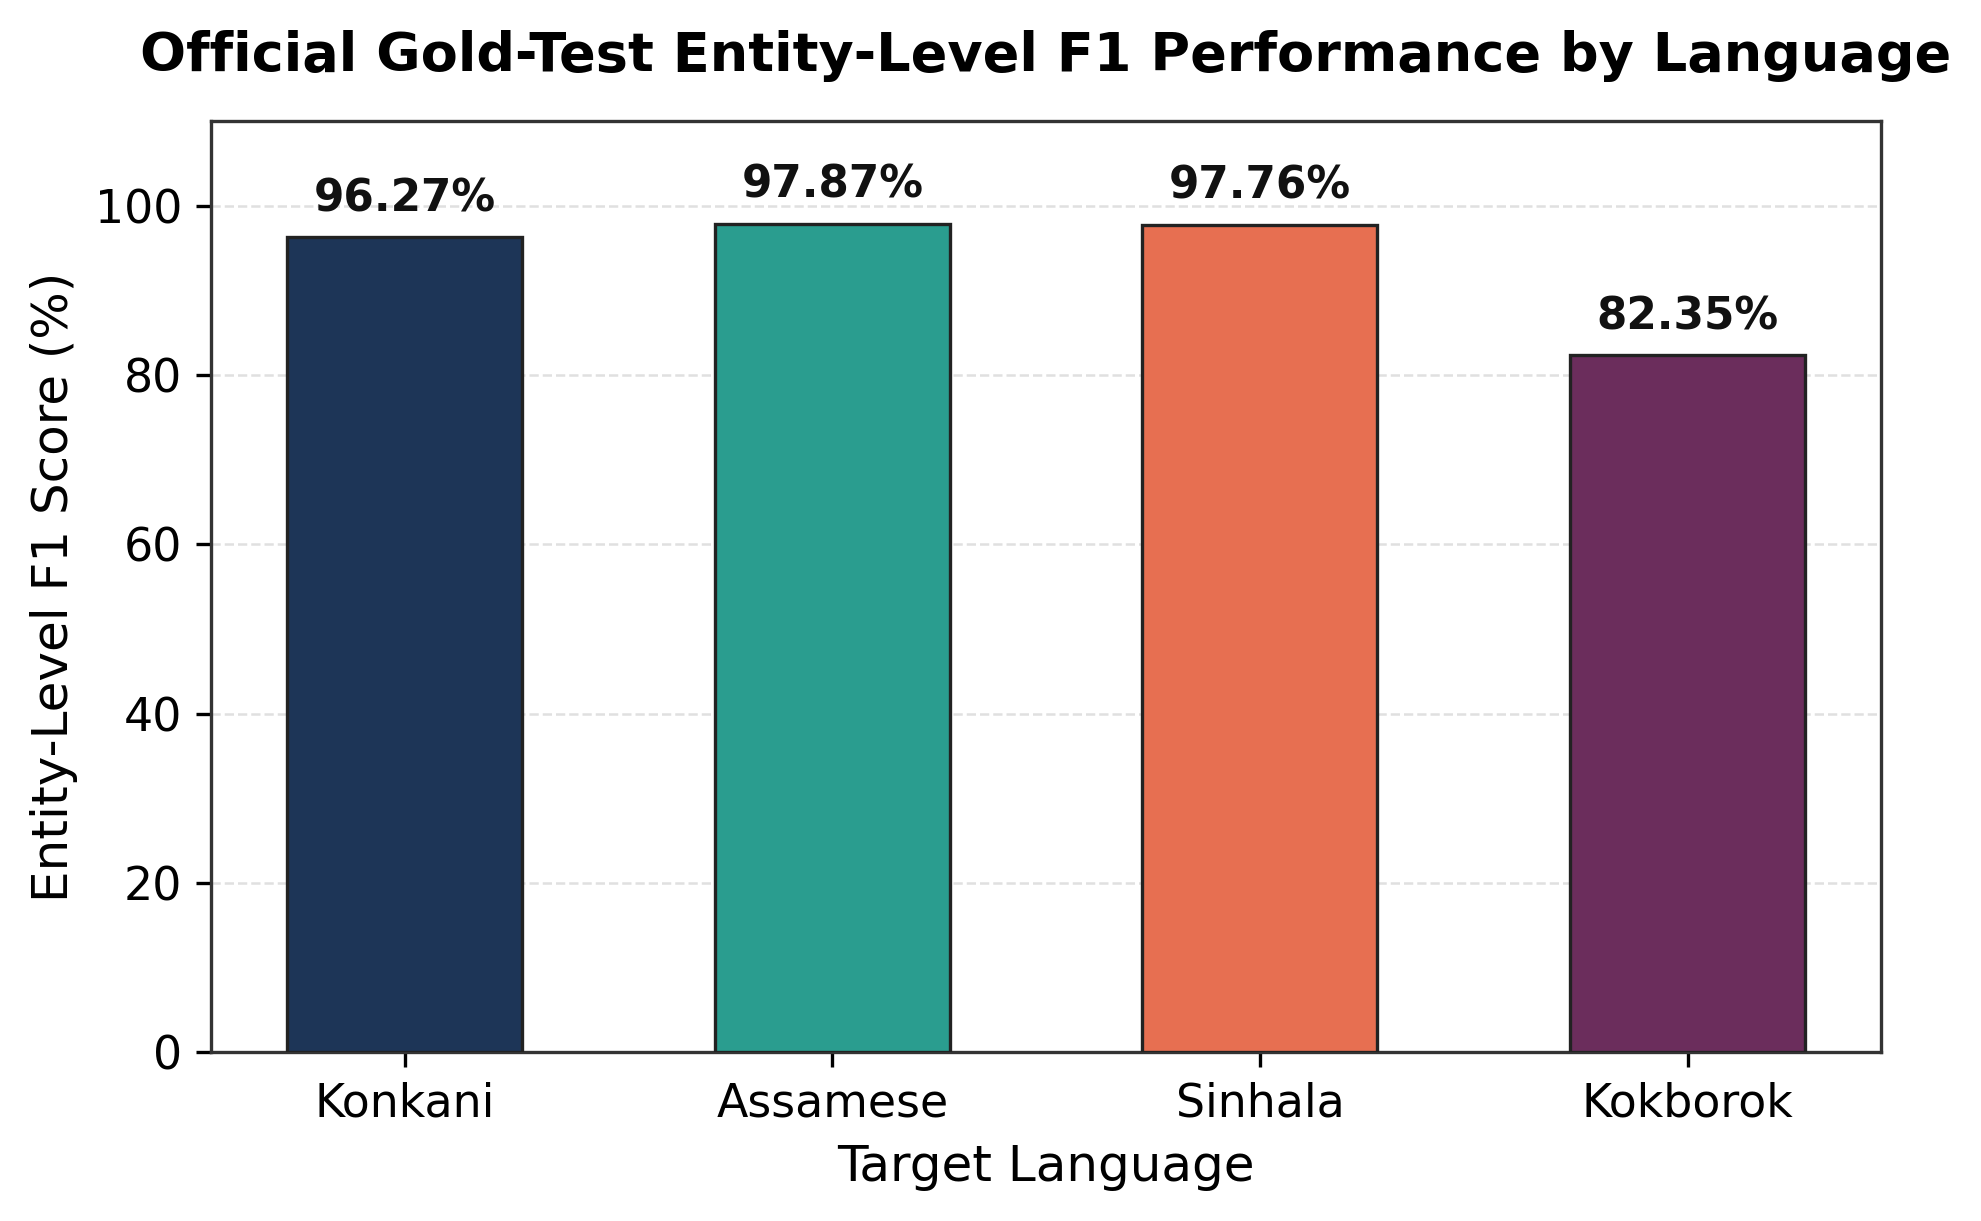
\includegraphics[width=0.72\columnwidth]{figures/fig_a_entity_f1.png}
\caption{Entity-level F1 performance of the proposed model on the official Gold-Test sets across the four target languages. Bars indicate exact span-level matching scores under CoNLL evaluation.}
\label{fig:entity_f1_bar}
\end{figure}

Figure~\ref{fig:entity_f1_bar} shows that three languages---Konkani (96.27\%), Assamese (97.87\%), and Sinhala (97.76\%)---attain entity F1 scores above 96\%, whereas Kokborok achieves 82.35\% on its locked test set. Crucially, token-level accuracy remains consistently high across all four languages, exceeding 99.4\% in every case (from 99.47\% in Konkani to 99.70\% in Sinhala, with Kokborok achieving 99.55\%). This difference demonstrates that token-level accuracy alone does not fully describe entity-level sequence labeling performance, as token accuracy is heavily dominated by majority Outside (\texttt{O}) tokens and does not reflect span boundary identification or entity classification difficulty.

To analyze the underlying precision and recall dynamics contributing to these F1 scores, Figure~\ref{fig:precision_recall_f1} provides a grouped breakdown of precision, recall, and F1 across the four languages.

\begin{figure}[htbp]
\centering
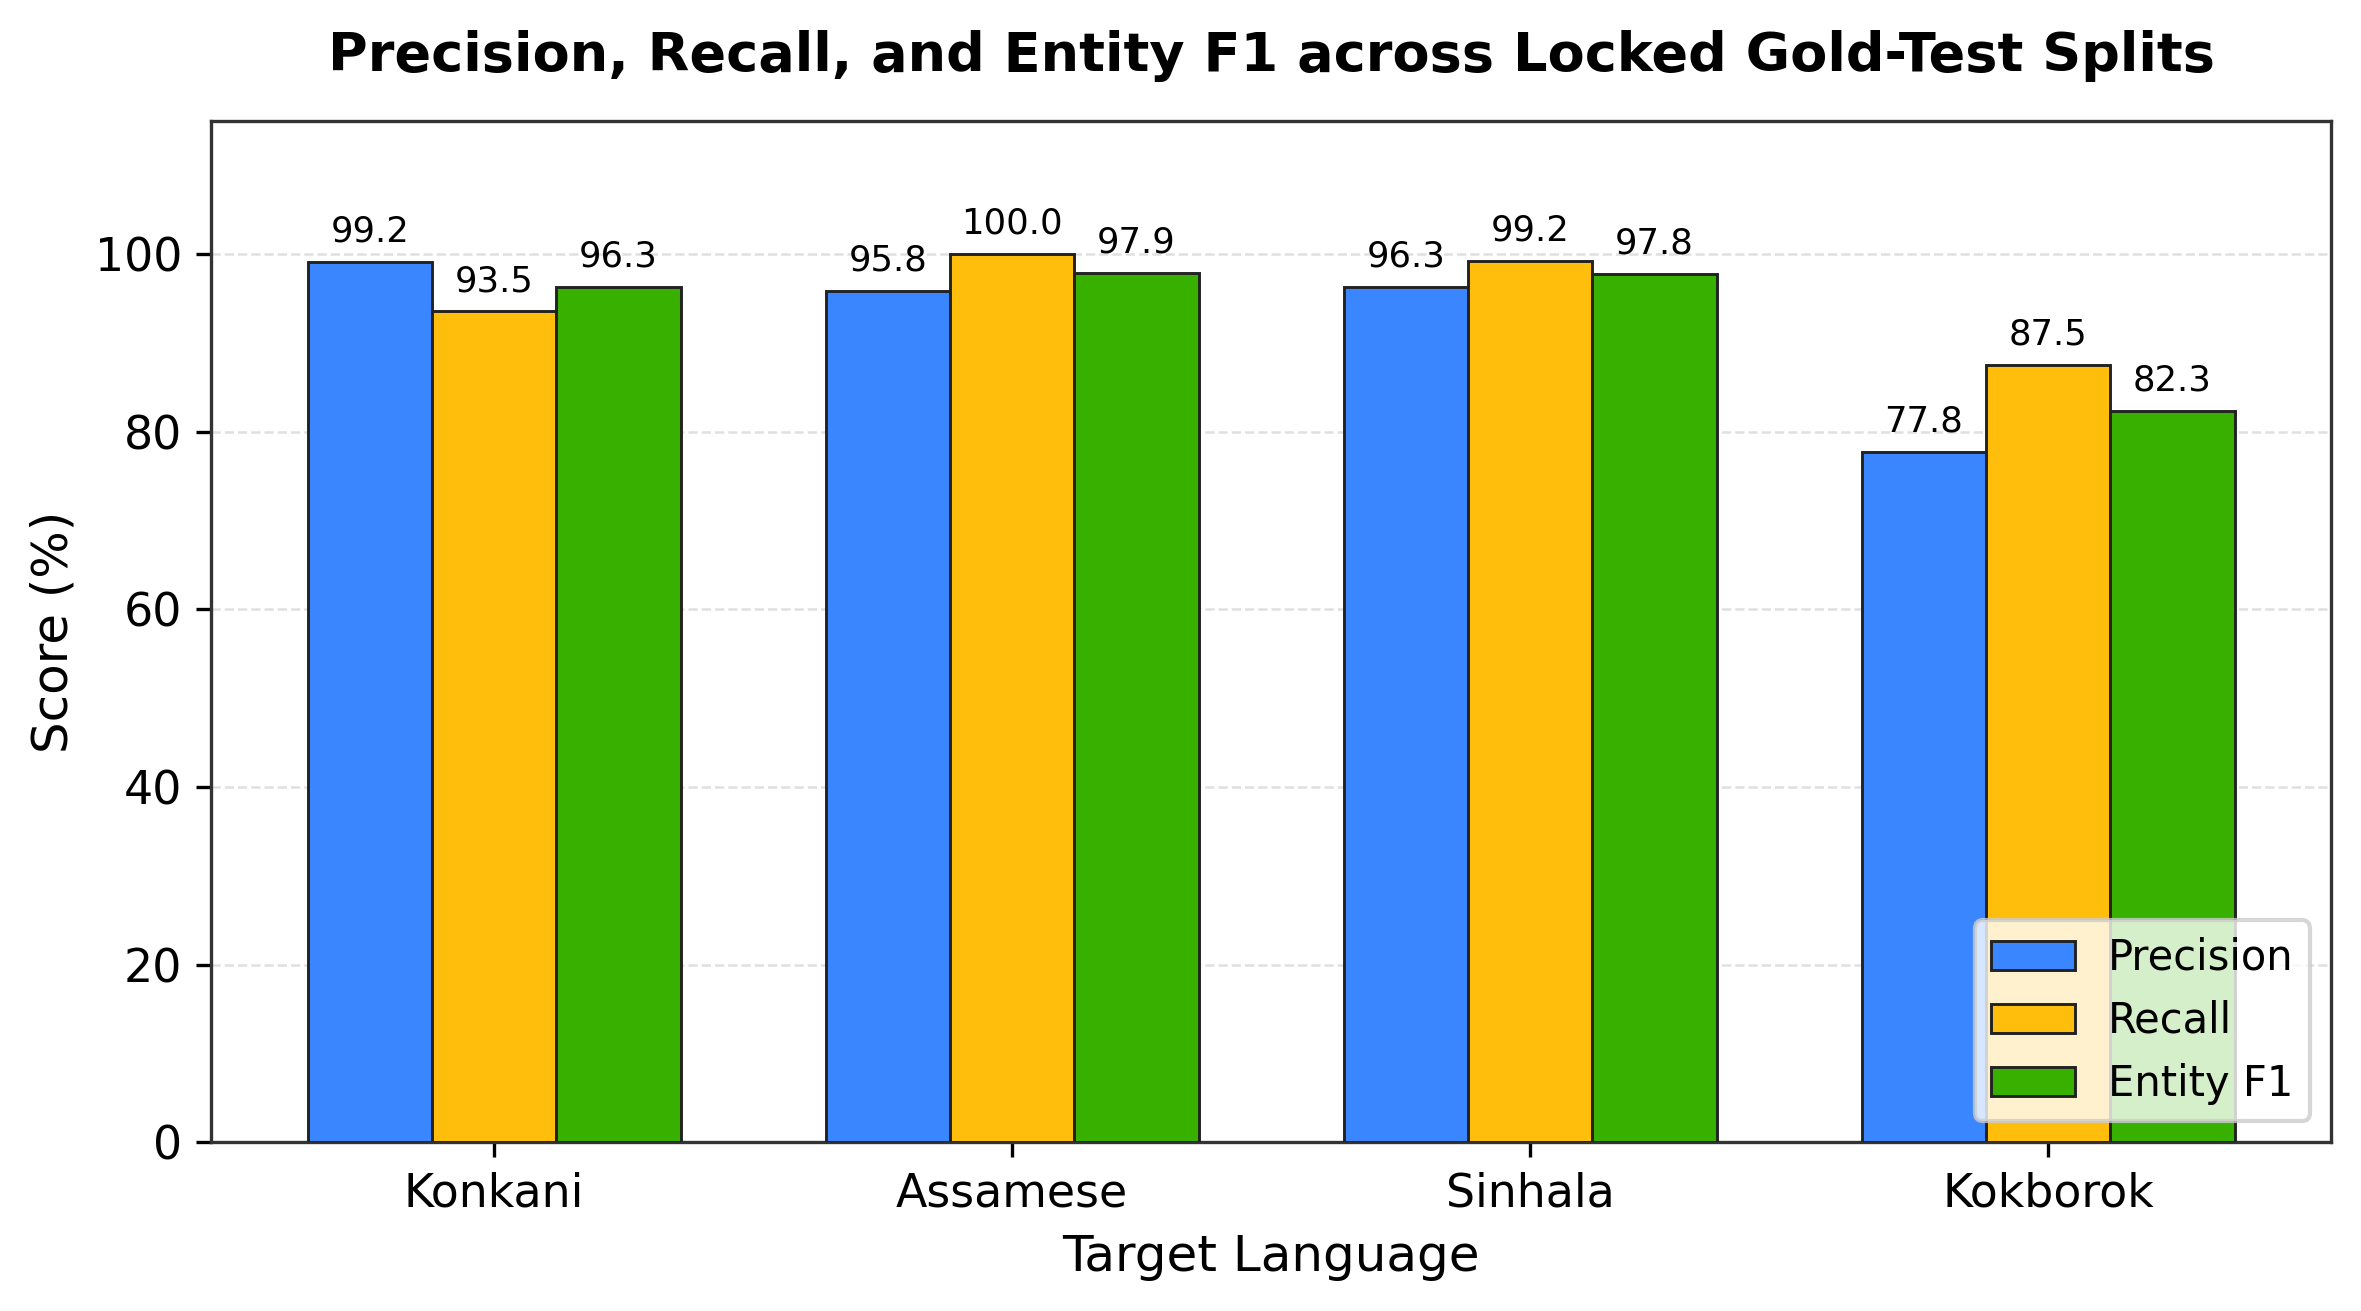
\includegraphics[width=0.86\columnwidth]{figures/fig_b_precision_recall_f1.png}
\caption{Grouped comparison of precision, recall, and entity-level F1 on the locked Gold-Test splits. Component metrics illustrate distinct trade-offs across orthographic settings.}
\label{fig:precision_recall_f1}
\end{figure}

The results in Figure~\ref{fig:precision_recall_f1} indicate that the four languages exhibit distinct error profiles. Assamese achieves 100.00\% recall across 138 gold test entities alongside 95.83\% precision. In contrast, Konkani exhibits high precision (99.15\%) with comparatively lower recall (93.55\%). Sinhala demonstrates balanced metrics, with 96.32\% precision and 99.24\% recall. Kokborok exhibits lower precision (77.78\%) and recall (87.50\%) than the other three languages. Examining precision and recall individually provides more diagnostic information regarding model behavior than relying solely on the single aggregate F1 metric.

\subsection{Language-Wise Performance}\label{subsec:lang_perf}

Table~\ref{tab:lang_breakdown} presents the detailed language-wise breakdown alongside the joint multilingual baseline comparisons recorded during training.

\begin{table}[htbp]
\centering
\caption{Language-Wise Performance on the Official Gold-Test Set and Joint Baseline Comparison}
\label{tab:lang_breakdown}
\footnotesize
\setlength{\tabcolsep}{3.5pt}
\begin{tabular}{lcccccc}
\toprule
\textbf{Language} & \textbf{Precision (\%)} & \textbf{Recall (\%)} & \textbf{Final F1 (\%)} & \textbf{Joint Baseline F1 (\%)} & \textbf{$\Delta$ (pp)} & \textbf{Accuracy (\%)} \\
\midrule
Konkani  & 99.15 & 93.55 & 96.27 & 95.87 & +0.40 & 99.47 \\
Assamese & 95.83 & 100.00 & 97.87 & 97.86 & +0.01 & 99.64 \\
Sinhala  & 96.32 & 99.24 & 97.76 & 97.04 & +0.72 & 99.70 \\
Kokborok & 77.78 & 87.50 & 82.35 & --- & --- & 99.55 \\
\bottomrule
\end{tabular}
\end{table}

To assess the effect of language-specific phased fine-tuning over the shared multilingual representation, Figure~\ref{fig:final_vs_joint_baseline} compares the final model against the joint multilingual baseline for the three languages where this baseline was evaluated.

\begin{figure}[htbp]
\centering
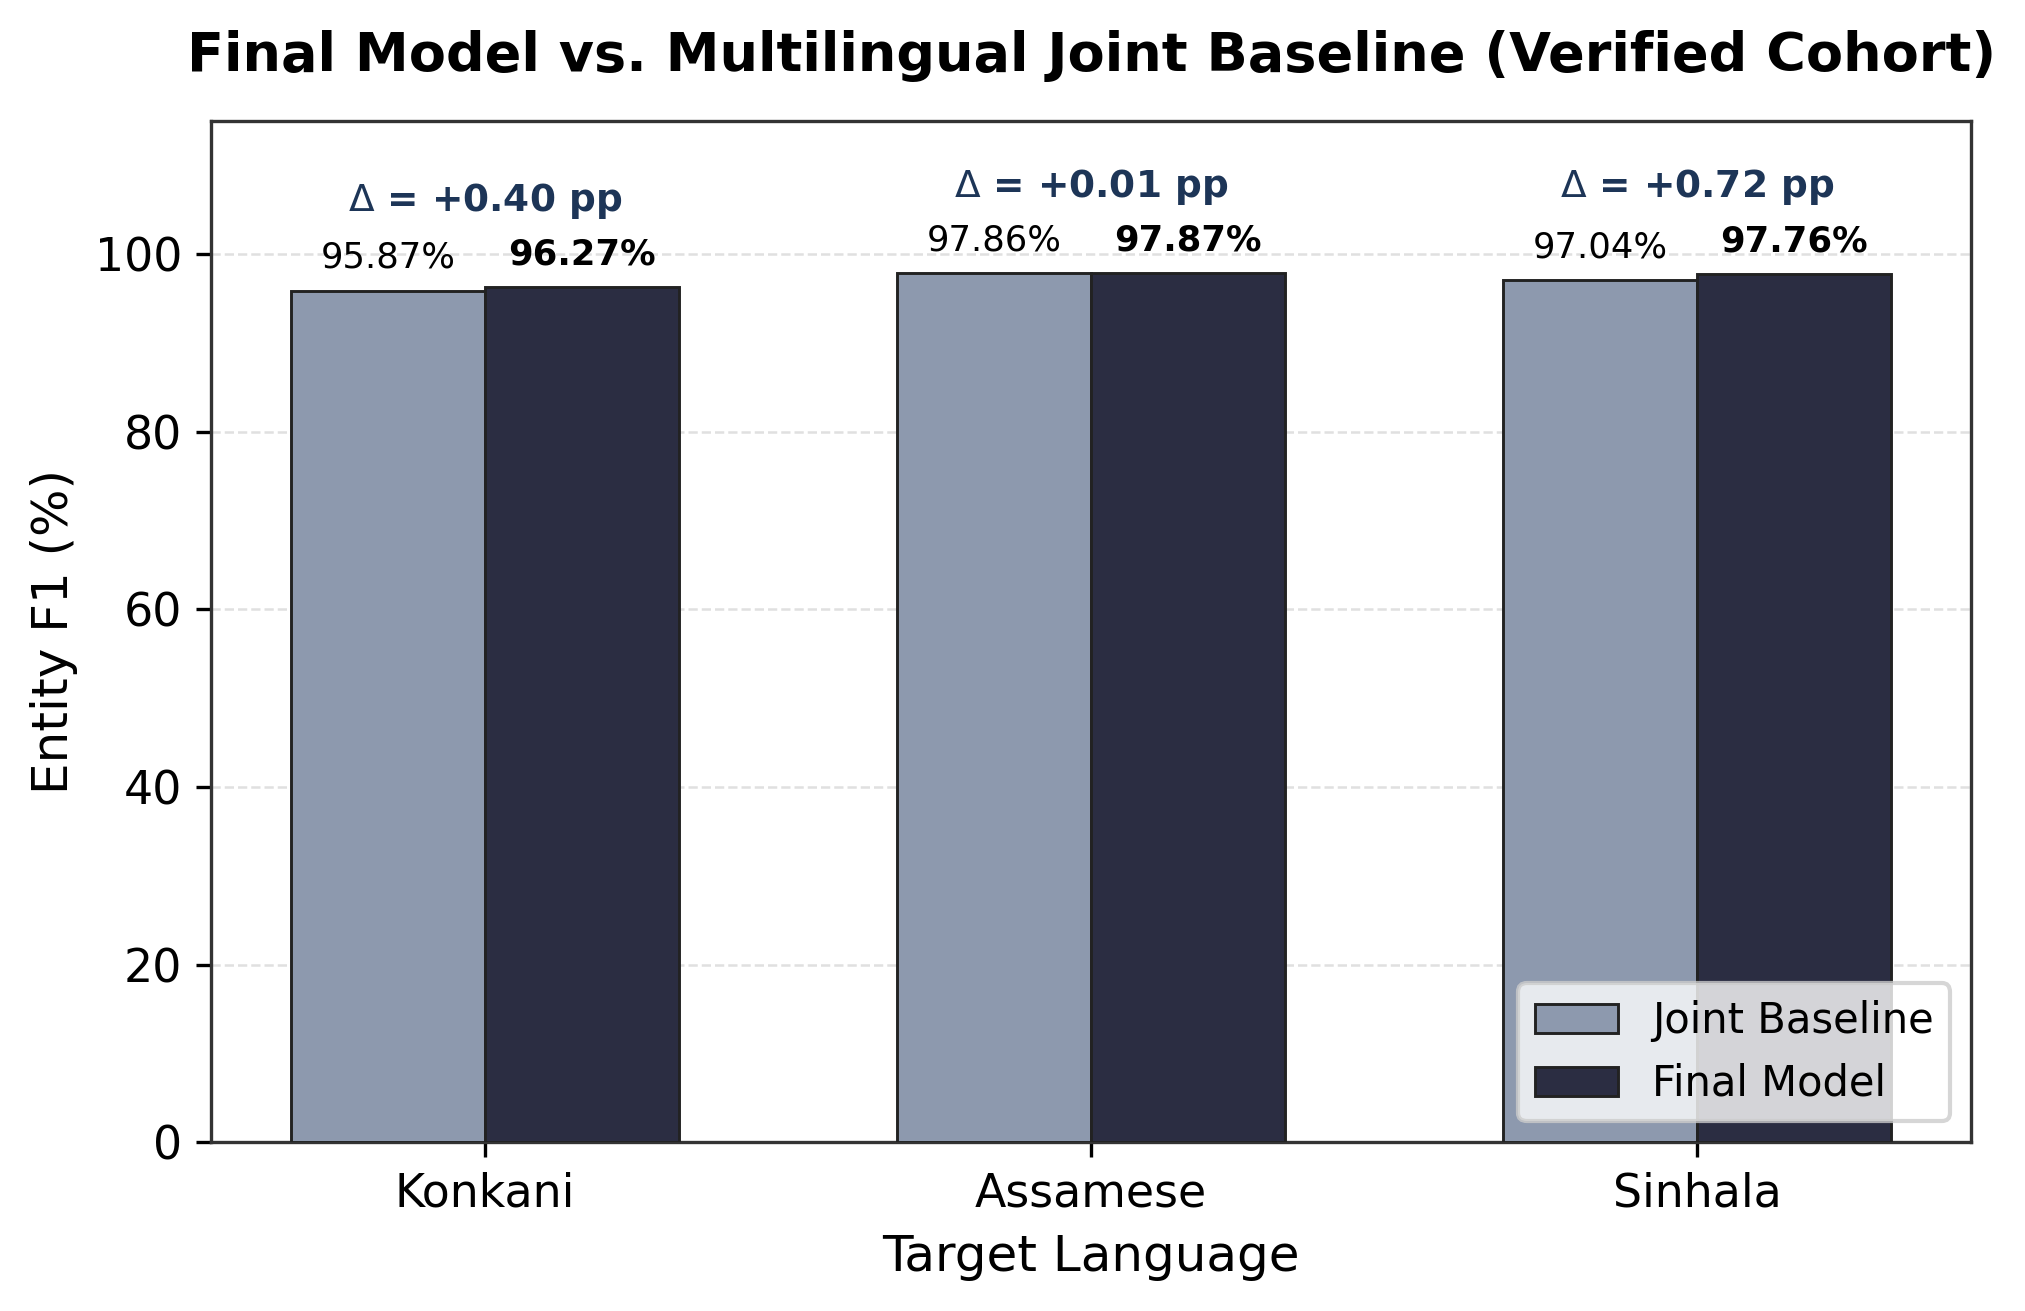
\includegraphics[width=0.76\columnwidth]{figures/fig_c_final_vs_joint_baseline.png}
\caption{Entity-level F1 comparison between the Multilingual Joint Baseline and the Final Model across Konkani, Assamese, and Sinhala. Kokborok is excluded because a joint baseline checkpoint was not recorded for it.}
\label{fig:final_vs_joint_baseline}
\end{figure}

Figure~\ref{fig:final_vs_joint_baseline} shows the measured percentage-point differences between the joint baseline and the final checkpoint: +0.40 percentage points (pp) in Konkani (from 95.87\% to 96.27\%), +0.01 pp in Assamese (from 97.86\% to 97.87\%), and +0.72 pp in Sinhala (from 97.04\% to 97.76\%). Kokborok is strictly excluded from this figure because no joint baseline checkpoint was recorded for it. The measured values reflect positive observed differences over the joint baseline for Konkani (+0.40 pp) and Sinhala (+0.72 pp), while Assamese performance remained essentially identical (+0.01 pp); these figures document the observed performance delta between checkpoints without asserting that unfreezing itself was isolated as the unique causal mechanism.

The raw prediction counts on the Gold-Test sets provide further empirical context:
\begin{itemize}
    \item \textbf{Konkani}: 116 true positives, 1 false positive, and 8 false negatives across 124 gold entity mentions.
    \item \textbf{Assamese}: 138 true positives, 6 false positives, and 0 false negatives across 138 gold entity mentions.
    \item \textbf{Sinhala}: 131 true positives, 5 false positives, and 1 false negative across 132 gold entity mentions.
    \item \textbf{Kokborok}: 14 true positives, 4 false positives, and 2 false negatives across 16 gold entity mentions.
\end{itemize}
Because the Kokborok test set contains only 16 annotated entities, each individual prediction error accounts for over 3 percentage points of the aggregate score.

\subsection{Model Configuration and Experimental Progression}\label{subsec:ablation_progression}

The project codebase defines four sequential architectural configurations to evaluate model components:
\begin{itemize}
    \item \textbf{Model 1 (Word Baseline)}: 100d learned word embedding, bidirectional LSTM context encoder with hidden size 128 per direction, linear emission layer, and CRF decoder.
    \item \textbf{Model 2 (Char-CNN)}: Augments Model 1 with character-level CNN convolutions (30 filters each for kernel widths 3, 4, 5) yielding a 190d composite representation ($100\text{d} + 90\text{d}$) and a two-layer BiLSTM.
    \item \textbf{Model 3 (Attention)}: Incorporates a 4-head self-attention layer with residual connection and Layer Normalization between the BiLSTM and the CRF decoder.
    \item \textbf{Model 4 (Proposed Multilingual Model)}: Adds the 16d language conditioning embedding to create the complete 206d composite input ($100\text{d} + 90\text{d} + 16\text{d}$) and decodes with a shared linear-chain CRF.
\end{itemize}

While all four configurations exist in the implementation, independent evaluation logs on the cryptographically locked Gold-Test splits were generated exclusively for the final multilingual system (Model 4). In accordance with strict scientific reporting principles, standalone F1 scores for Models 1--3 are not claimed. The architecture is evaluated and analyzed as a composite system.

\subsection{Explainability and Attention Attribution Analysis}\label{subsec:explainability_analysis}

A central objective of this research is examining whether internal self-attention distributions provide faithful decision explanations for low-resource sequence labeling. Two attribution formulations were evaluated: Raw Attention and Gradient $\times$ Attention. To examine how attention distributes across individual input tokens, Figure~\ref{fig:attribution_heatmap} visualizes the token-level attribution weights generated by the model on an actual Gold-Development instance.

\begin{figure}[htbp]
\centering
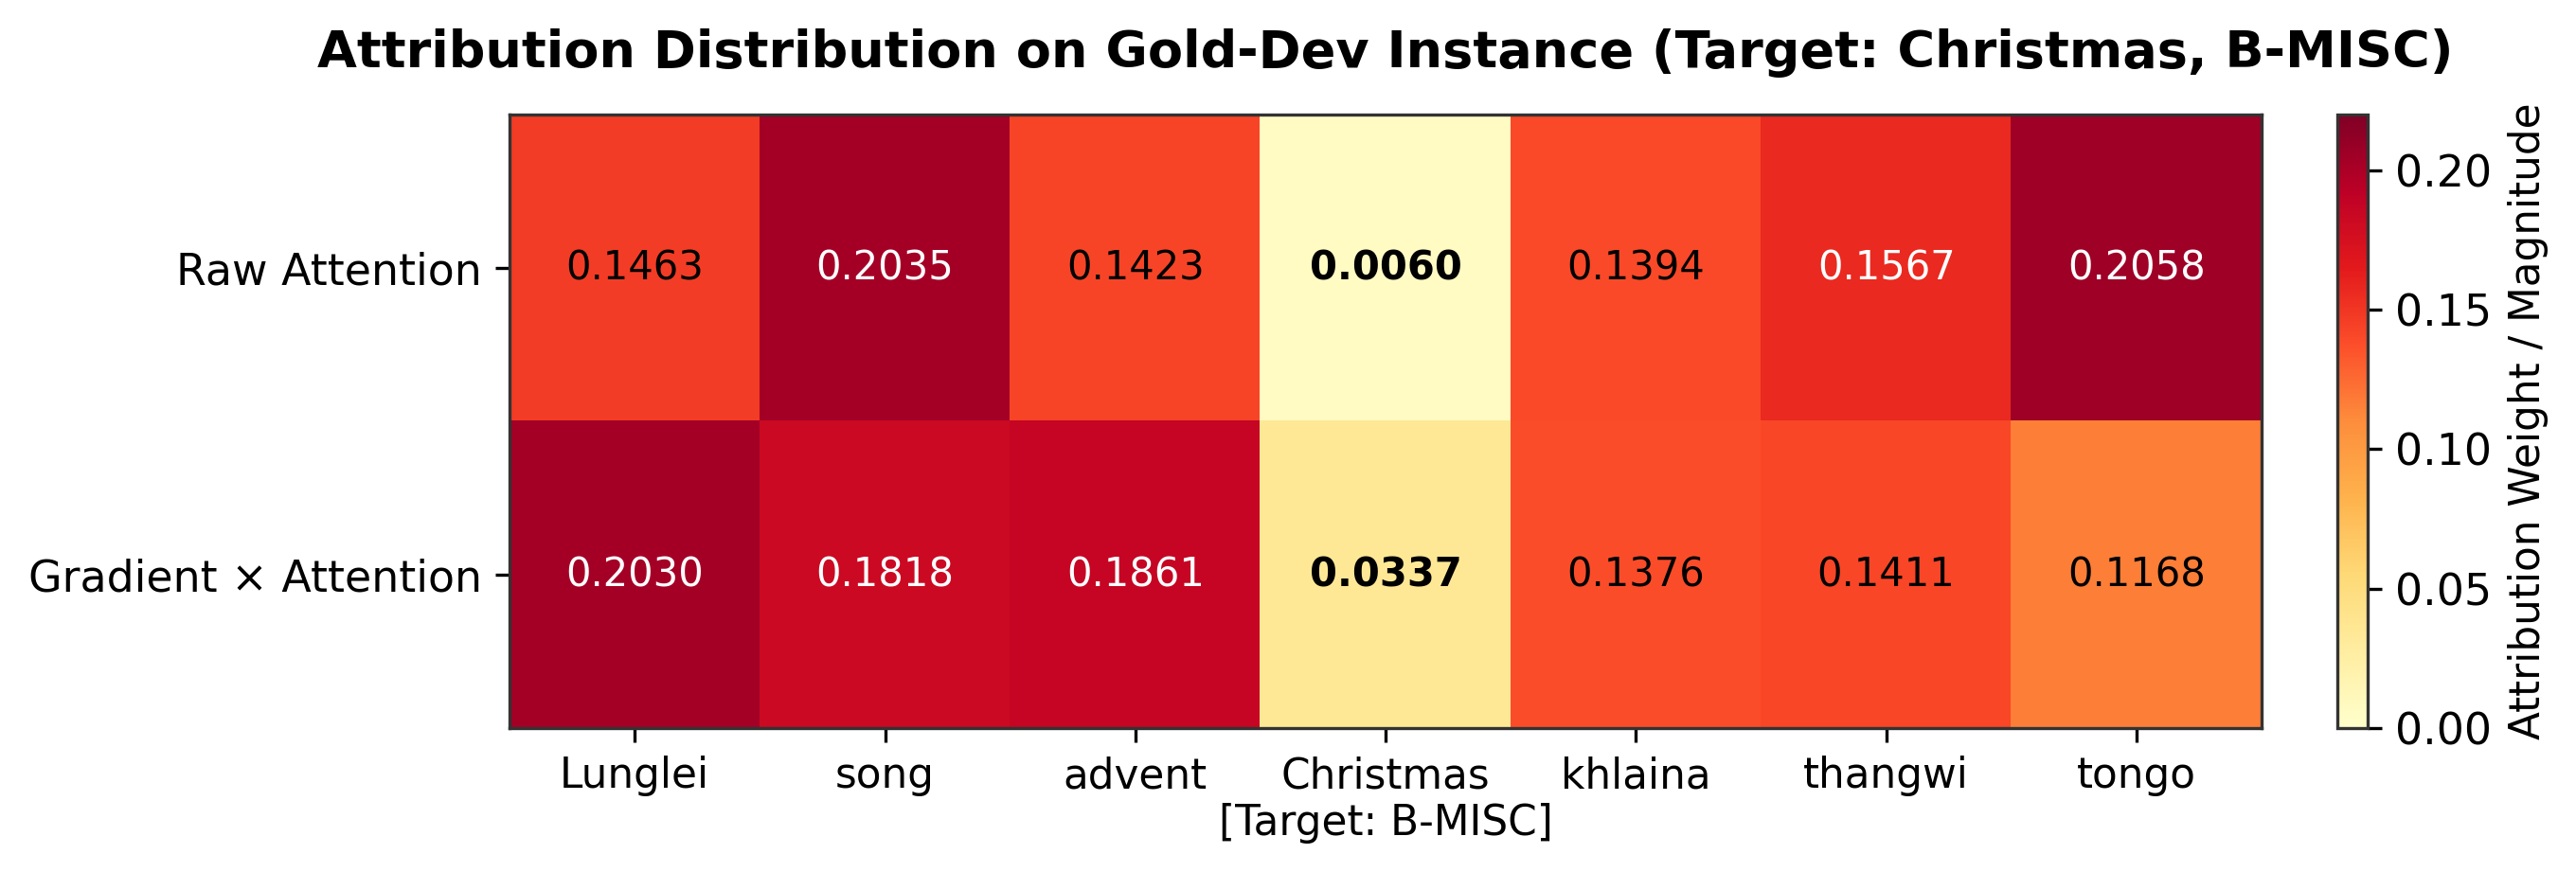
\includegraphics[width=0.92\columnwidth]{figures/fig_d_attribution_heatmap.png}
\caption{Attribution heatmap for an actual Gold-Development prediction (Language: Kokborok, target entity query: \textit{Christmas}, Gold: \texttt{B-MISC}). Numeric cell values show normalized attribution weights under Raw Attention and Gradient $\times$ Attention. Attribution values represent internal model weights and gradient sensitivity, not causal proof of decision mechanisms.}
\label{fig:attribution_heatmap}
\end{figure}

Figure~\ref{fig:attribution_heatmap} shows that for the target entity token \textit{Christmas} (position 3), both Raw Attention (0.0060) and Gradient $\times$ Attention (0.0337) allocate low attribution mass to the target entity itself. Instead, substantial attribution is assigned to surrounding contextual tokens, including sentence-initial tokens (\textit{Lunglei}: 0.1463 Raw, 0.2030 Grad $\times$ Attn) and verbal heads (\textit{song}: 0.2035 Raw, 0.1818 Grad $\times$ Attn; \textit{tongo}: 0.2058 Raw, 0.1168 Grad $\times$ Attn). These values demonstrate that the attribution layer distributes weight across broader contextual positions rather than isolating the entity query token.

\textbf{Target-Token Attribution Audit.} To evaluate whether this diffuse attribution pattern holds systematically across predictions, an attribution audit was conducted across all correctly predicted Gold-Development entity instances ($N=125$ for Konkani, $N=139$ for Assamese, and $N=131$ for Sinhala). Table~\ref{tab:target_token_audit} reports the audit statistics.

\begin{table}[htbp]
\centering
\caption{Target-Token Attribution Audit across Gold-Development Entity Predictions}
\label{tab:target_token_audit}
\scriptsize
\setlength{\tabcolsep}{3.5pt}
\begin{tabular}{llcccccc}
\toprule
\textbf{Language} & \textbf{Method} & \textbf{$N$} & \textbf{Mean Attr.} & \textbf{\% $\le$ 0.001} & \textbf{Top-1 (\%)} & \textbf{Top-3 (\%)} & \textbf{Mean Rank} \\
\midrule
\multirow{2}{*}{Konkani}  & Gradient $\times$ Attn & 125 & 0.003278 & 92.80 & 0.00 & 1.60 & 16.94 \\
                          & Raw Attention          & 125 & 0.002845 & 93.60 & 0.00 & 0.80 & 17.26 \\
\midrule
\multirow{2}{*}{Assamese} & Gradient $\times$ Attn & 139 & 0.002364 & 98.56 & 0.72 & 1.44 & 17.17 \\
                          & Raw Attention          & 139 & 0.000969 & 98.56 & 0.00 & 0.00 & 17.30 \\
\midrule
\multirow{2}{*}{Sinhala}  & Gradient $\times$ Attn & 131 & 0.000204 & 98.47 & 0.00 & 0.00 & 20.57 \\
                          & Raw Attention          & 131 & 0.000043 & 99.24 & 0.00 & 0.00 & 20.63 \\
\bottomrule
\end{tabular}
\end{table}

To analyze the degree of attribution sparsity across languages, Figure~\ref{fig:target_token_near_zero} plots the percentage of target entity tokens receiving near-zero attribution mass ($\le 0.001$).

\begin{figure}[htbp]
\centering
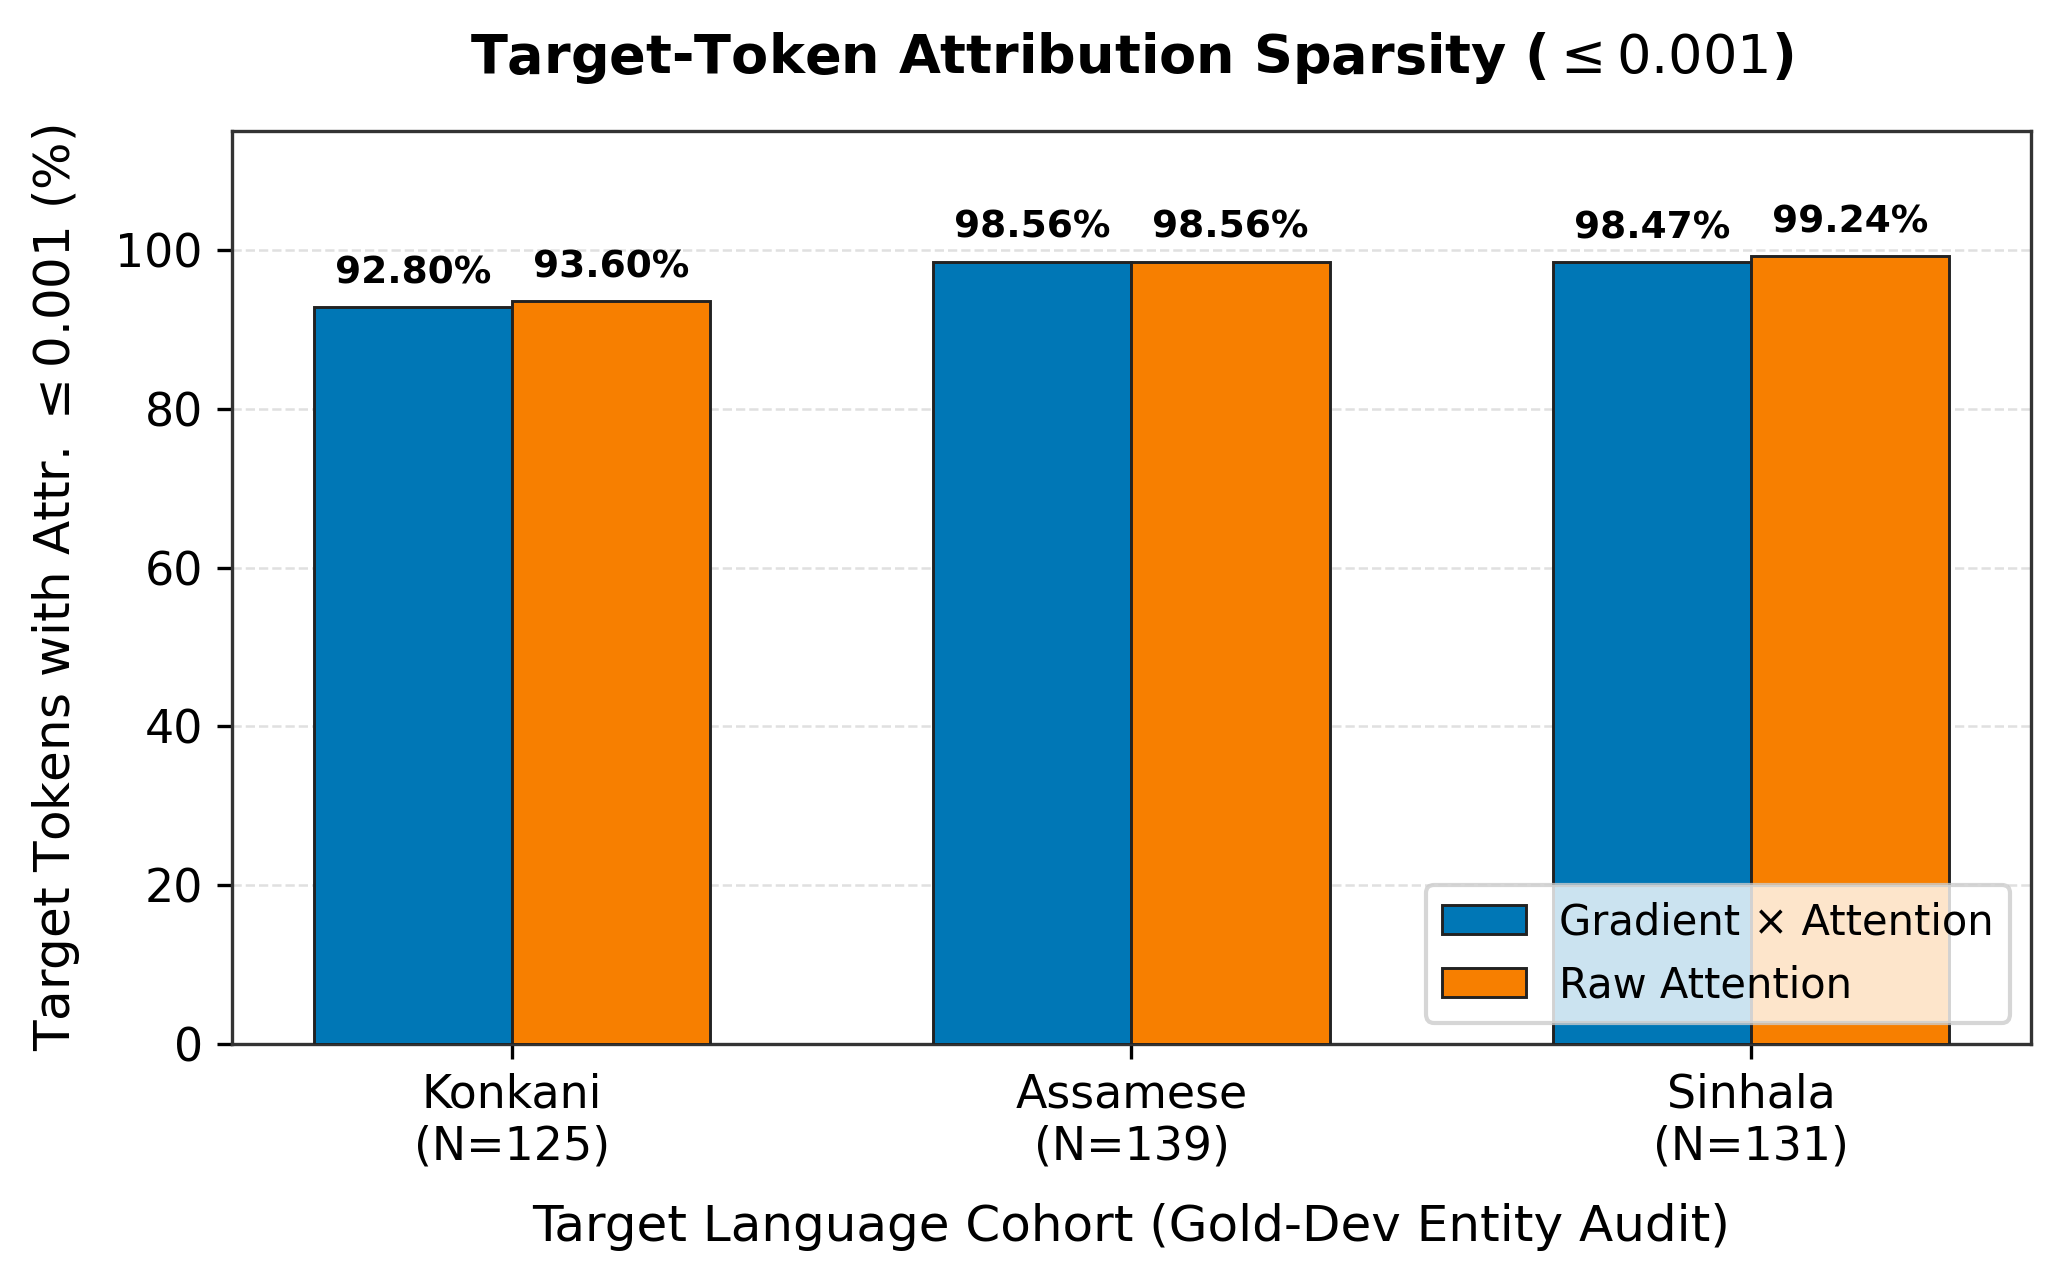
\includegraphics[width=0.76\columnwidth]{figures/fig_e_target_token_near_zero.png}
\caption{Proportion of target entity tokens receiving near-zero attribution mass ($\le 0.001$) across correctly predicted Gold-Development entities in Konkani ($N=125$), Assamese ($N=139$), and Sinhala ($N=131$).}
\label{fig:target_token_near_zero}
\end{figure}

As shown in Figure~\ref{fig:target_token_near_zero}, over 92\% of target entity tokens receive attribution scores below 0.001 under both methods across all three evaluated languages, reaching 98.56\% in Assamese and 99.24\% in Sinhala. To examine where target tokens rank within overall sentence attributions, Figure~\ref{fig:target_token_rank} displays the mean rank of target entity tokens under contextual attribution ordering.

\begin{figure}[htbp]
\centering
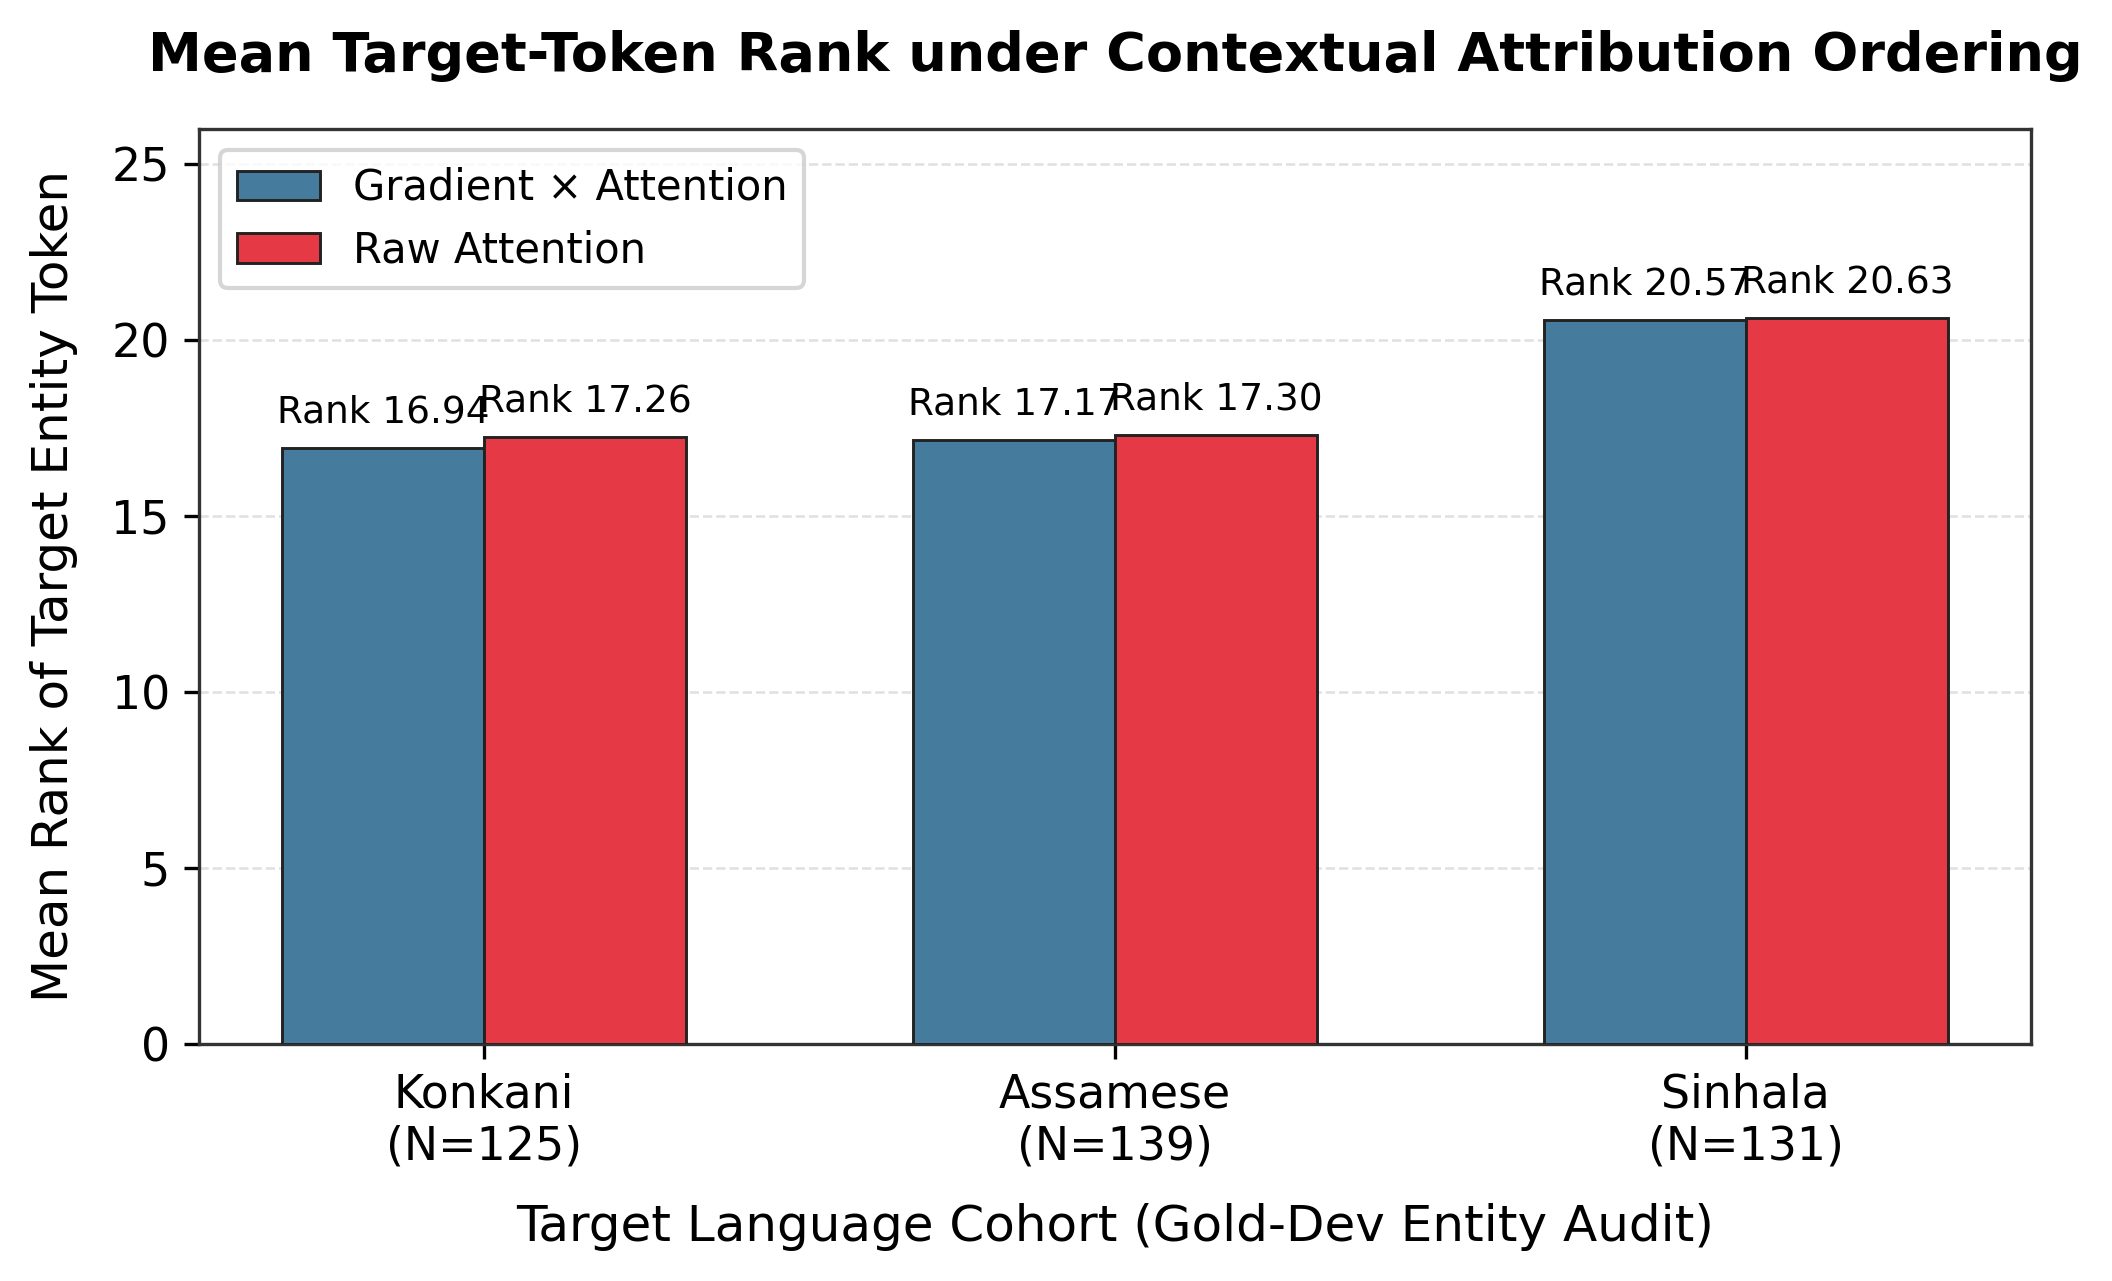
\includegraphics[width=0.76\columnwidth]{figures/fig_f_target_token_rank.png}
\caption{Mean rank of target entity tokens within sentence-level attribution orderings (where rank 1 corresponds to the highest attributed token in the sentence).}
\label{fig:target_token_rank}
\end{figure}

Figure~\ref{fig:target_token_rank} demonstrates that target tokens appear late in sentence attribution rankings, with mean ranks ranging between 16.94 and 20.63. The attribution audit demonstrates that high entity-level NER performance is not accompanied by the concentration of attention on the target token itself. Structurally, this behavior is consistent with the placement of the two-layer bidirectional LSTM encoder prior to the self-attention layer. Because the recurrent states already encode contextual information from preceding and subsequent tokens before entering the attention block, the attention mechanism operates on context-rich representations. Consequently, high classification accuracy does not require attention weights to concentrate directly on the target entity token.

\subsection{Faithfulness Evaluation}\label{subsec:faithfulness_eval}

To determine whether attribution scores reflect context tokens that influence model predictions, we evaluate faithfulness through an empirical token-erasure benchmark.

\textbf{Erasure Protocol.} The erasure experiment evaluates whether tokens receiving higher attribution are associated with larger confidence changes under controlled perturbation. Evaluated on Gold-Development entity predictions (100 instances each for Konkani, Assamese, and Sinhala; all 17 available instances for Kokborok), the primary protocol neutralizes context tokens by setting their 206-dimensional composite input embeddings to zero ($\mathbf{x}_j = \mathbf{0}$). To evaluate contextual attribution fairly, the target query token $q$ is strictly excluded from both top-$k$ and random-$k$ candidate pools ($j \neq q$). Prediction confidence is computed as the exact posterior marginal probability under forward-backward linear-chain CRF inference:
\begin{equation}
C_0 = P_{\text{CRF}}(y_q = y^*_q \mid \mathbf{x}).
\end{equation}
When top-$k$ context tokens are zeroed, the resulting confidence drop $\Delta_{\text{top-}k} = \max(0, C_0 - C_{\text{top-}k})$ is compared against the drop from zeroing random-$k$ context tokens $\Delta_{\text{rand-}k}$. The faithfulness deletion gap is defined as:
\begin{equation}
\Delta_k = \Delta_{\text{top-}k} - \Delta_{\text{rand-}k}.
\end{equation}
A positive gap indicates that zeroing top-attributed context tokens degrades prediction confidence more than zeroing random context tokens. Table~\ref{tab:faithfulness_results} presents the authoritative empirical results from Phase 15.

\begin{table}[htbp]
\centering
\caption{Faithfulness Evaluation under the Primary Token-Erasure Protocol (Zero-Embedding with CRF Marginals)}
\label{tab:faithfulness_results}
\footnotesize
\setlength{\tabcolsep}{4.5pt}
\begin{tabular}{llcccc}
\toprule
\textbf{Language} & \textbf{Attribution Method} & \textbf{$k$} & \textbf{Mean Top Drop} & \textbf{Mean Rand Drop} & \textbf{Faithfulness Gap ($\Delta_k$)} \\
\midrule
\multirow{6}{*}{Konkani}  & \multirow{3}{*}{Raw Attention} 
                            & 1 & 0.0665 & 0.0302 & \textbf{+0.0363} \\
                          & & 2 & 0.1039 & 0.0627 & \textbf{+0.0412} \\
                          & & 3 & 0.1315 & 0.0999 & \textbf{+0.0316} \\
\cmidrule{2-6}
                          & \multirow{3}{*}{Gradient $\times$ Attn} 
                            & 1 & 0.0492 & 0.0302 & +0.0190 \\
                          & & 2 & 0.0877 & 0.0627 & +0.0250 \\
                          & & 3 & 0.1126 & 0.0999 & +0.0127 \\
\midrule
\multirow{6}{*}{Assamese} & \multirow{3}{*}{Raw Attention} 
                            & 1 & 0.0416 & 0.0551 & -0.0135 \\
                          & & 2 & 0.0704 & 0.0855 & -0.0150 \\
                          & & 3 & 0.0979 & 0.1109 & -0.0130 \\
\cmidrule{2-6}
                          & \multirow{3}{*}{Gradient $\times$ Attn} 
                            & 1 & 0.0319 & 0.0551 & -0.0232 \\
                          & & 2 & 0.0635 & 0.0855 & -0.0220 \\
                          & & 3 & 0.0967 & 0.1109 & -0.0143 \\
\midrule
\multirow{6}{*}{Sinhala}  & \multirow{3}{*}{Raw Attention} 
                            & 1 & 0.0379 & 0.0272 & \textbf{+0.0107} \\
                          & & 2 & 0.0652 & 0.0663 & -0.0011 \\
                          & & 3 & 0.0943 & 0.0915 & \textbf{+0.0029} \\
\cmidrule{2-6}
                          & \multirow{3}{*}{Gradient $\times$ Attn} 
                            & 1 & 0.0330 & 0.0272 & +0.0058 \\
                          & & 2 & 0.0583 & 0.0663 & -0.0080 \\
                          & & 3 & 0.0864 & 0.0915 & -0.0051 \\
\midrule
\multirow{6}{*}{Kokborok} & \multirow{3}{*}{Raw Attention} 
                            & 1 & 0.0033 & 0.0165 & -0.0132 \\
                          & & 2 & 0.0200 & 0.0399 & -0.0198 \\
                          & & 3 & 0.0299 & 0.0680 & -0.0381 \\
\cmidrule{2-6}
                          & \multirow{3}{*}{Gradient $\times$ Attn} 
                            & 1 & 0.0024 & 0.0165 & -0.0141 \\
                          & & 2 & 0.0034 & 0.0399 & -0.0365 \\
                          & & 3 & 0.0141 & 0.0680 & -0.0539 \\
\bottomrule
\end{tabular}
\end{table}

To visualize how faithfulness gaps evolve as more context tokens are removed, Figure~\ref{fig:faithfulness_line} shows the gap trajectories across $k \in \{1, 2, 3\}$ for each language.

\begin{figure}[htbp]
\centering
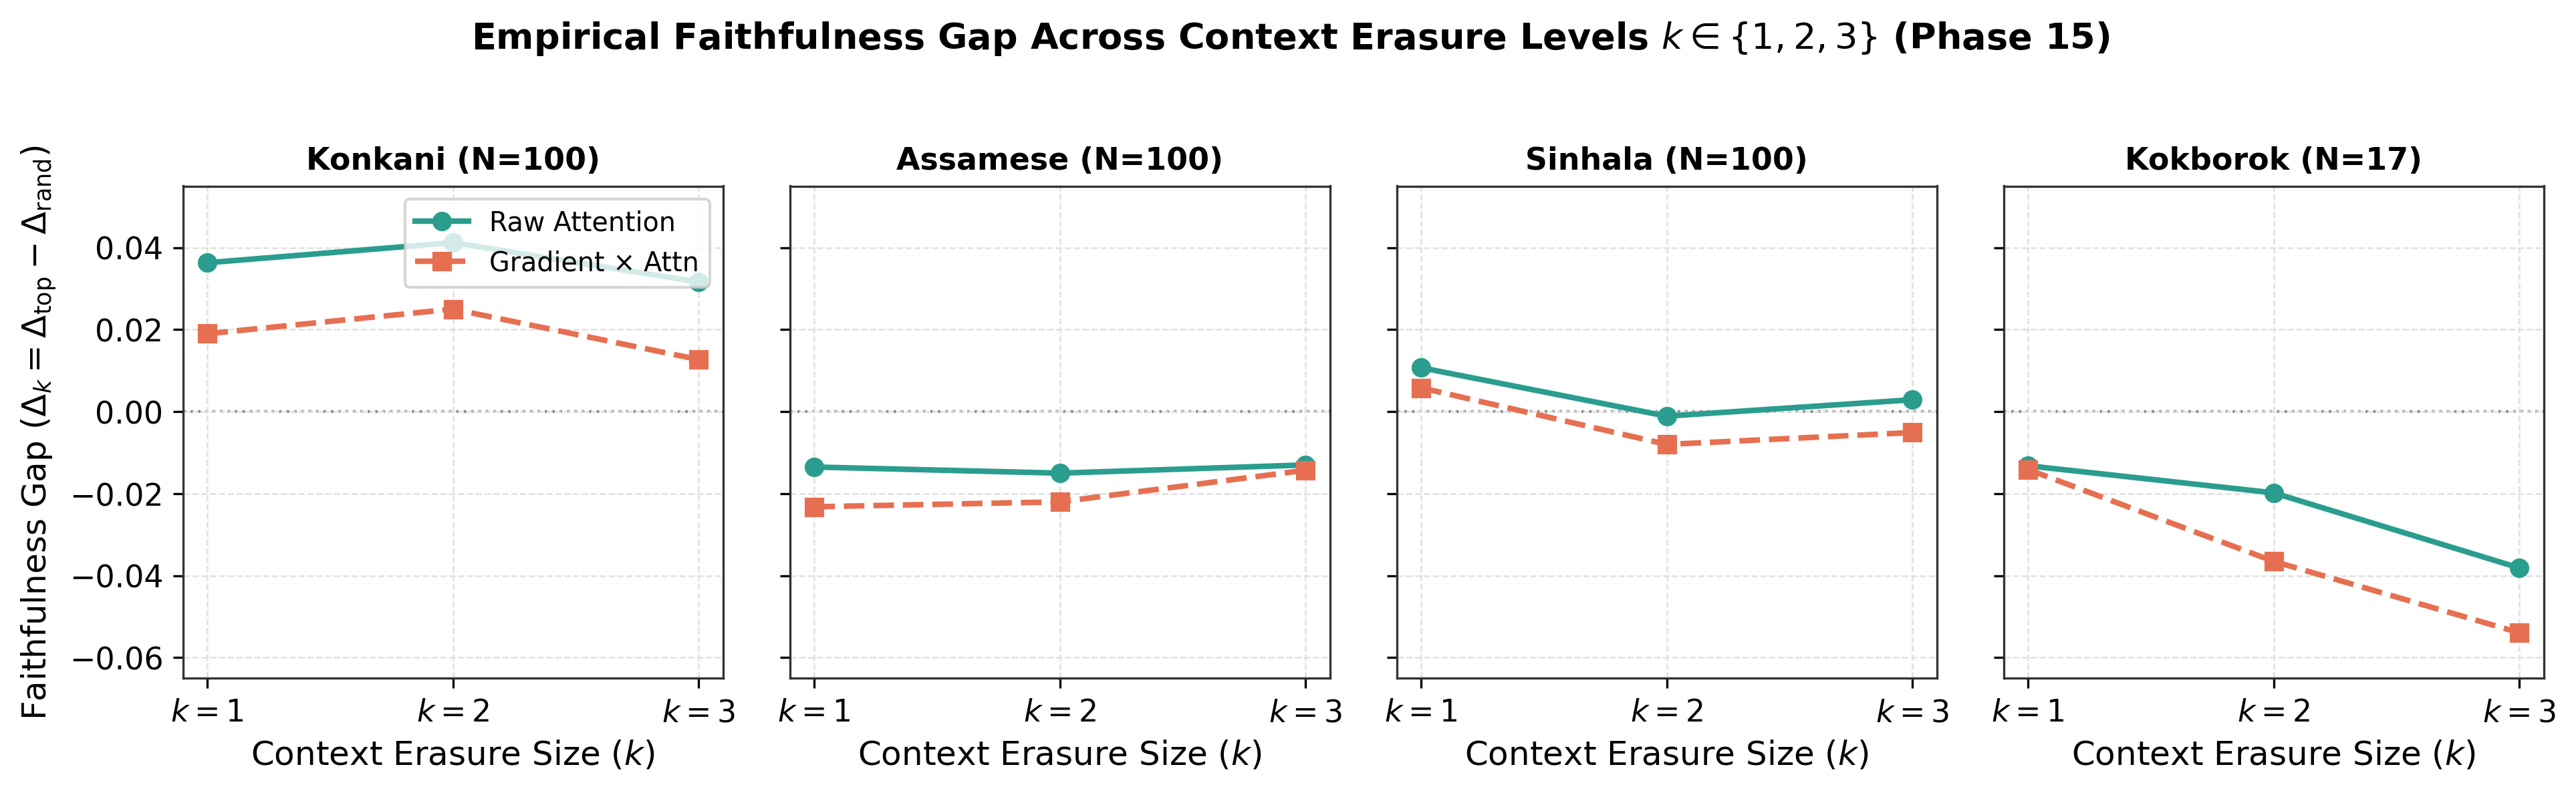
\includegraphics[width=\columnwidth]{figures/fig_g_faithfulness_line.png}
\caption{Faithfulness gap trajectories across context erasure sizes $k \in \{1, 2, 3\}$ for Raw Attention and Gradient $\times$ Attention across the four languages. The dotted line at $\Delta_k = 0$ denotes parity between top-$k$ and random-$k$ erasure.}
\label{fig:faithfulness_line}
\end{figure}

To provide a direct cross-language comparison across methods and context erasure levels, Figure~\ref{fig:faithfulness_heatmap} displays the summary heatmap.

\begin{figure}[htbp]
\centering
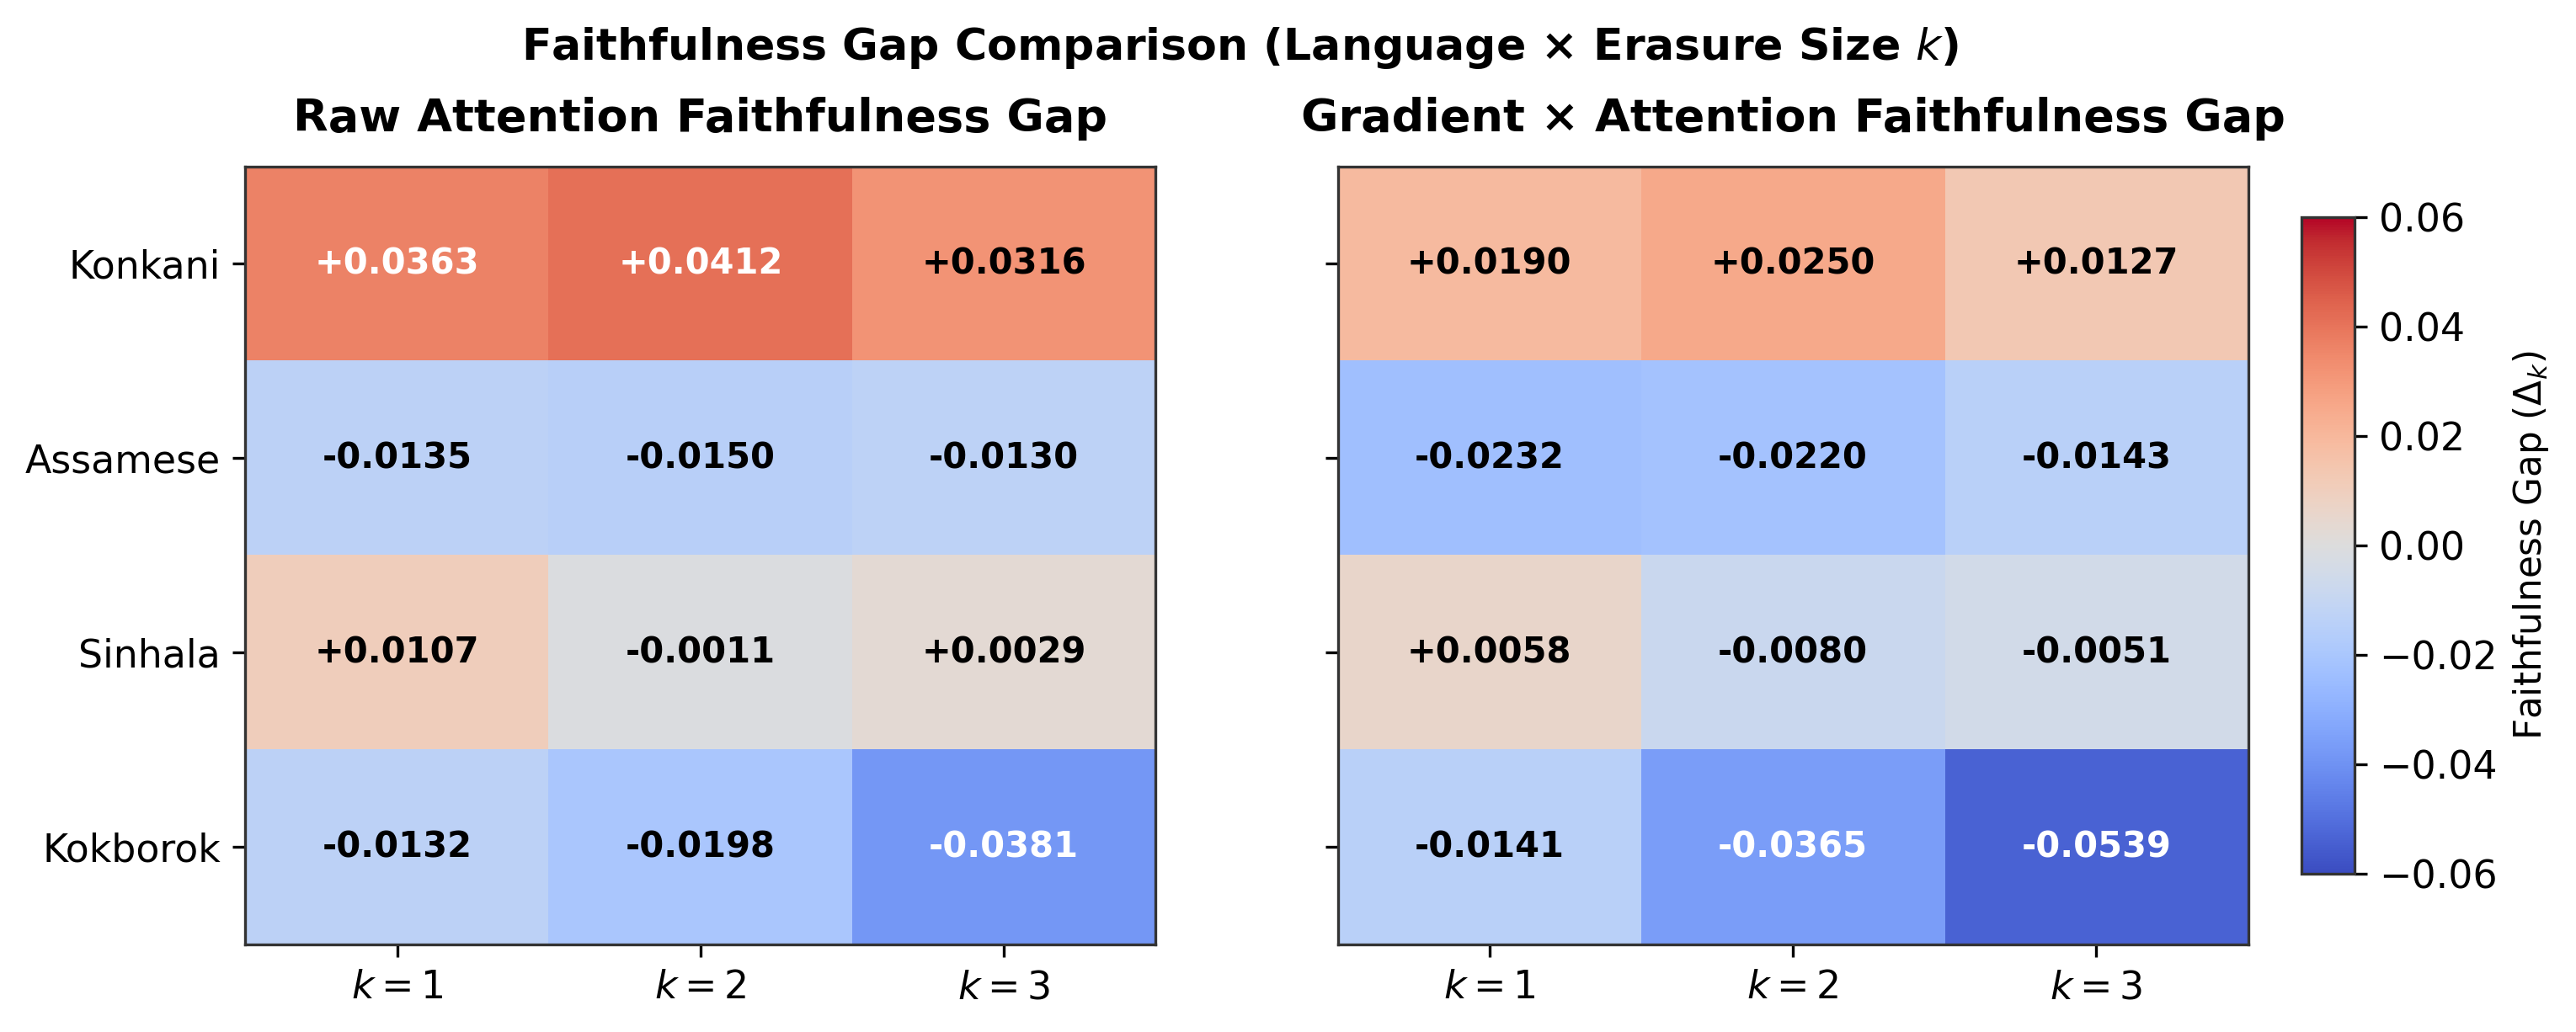
\includegraphics[width=0.90\columnwidth]{figures/fig_h_faithfulness_heatmap.png}
\caption{Compact heatmap comparison of faithfulness gaps across languages, attribution methods, and context erasure levels $k \in \{1, 2, 3\}$. Color scale ranges from $-0.06$ (blue) to $+0.06$ (red).}
\label{fig:faithfulness_heatmap}
\end{figure}

Figure~\ref{fig:faithfulness_line} and Figure~\ref{fig:faithfulness_heatmap} show distinct empirical behavior across languages. In Konkani, both Raw Attention and Gradient $\times$ Attention produce consistently positive faithfulness gaps across all $k$ ($\Delta_k = +0.0127$ to $+0.0412$), with Raw Attention attaining win rates of 72.0\% at $k=1$, 63.0\% at $k=2$, and 61.0\% at $k=3$. In Sinhala, gaps are modestly positive at $k=1$ (+0.0107 for Raw Attention, +0.0058 for Gradient $\times$ Attention) and near zero at $k=2$ and $k=3$. Conversely, Assamese and Kokborok exhibit negative faithfulness gaps across all evaluated $k$ values (e.g., $\Delta_k = -0.0130$ to $-0.0232$ in Assamese; $\Delta_k = -0.0132$ to $-0.0539$ in Kokborok).

A negative faithfulness gap indicates that zeroing tokens selected by the attribution method resulted in a smaller reduction in CRF marginal confidence than zeroing random context tokens. One possible explanation is that, because the attention layer operates on recurrently contextualized representations, perturbing arbitrary context tokens may alter the BiLSTM-derived representations more broadly than perturbing tokens selected by the post-recurrent attribution mechanism. These results therefore indicate that attention attribution should not be assumed to provide faithful causal explanations without empirical validation.

\subsection{Kokborok Resource-Limited Analysis}\label{subsec:kokborok_eval}

Kokborok represents the most resource-constrained setting in this study. On the official locked Gold-Test split, the final model achieves:
\begin{itemize}
    \item \textbf{Precision}: 77.78\%
    \item \textbf{Recall}: 87.50\%
    \item \textbf{Entity F1}: 82.35\%
    \item \textbf{Token Accuracy}: 99.55\%
\end{itemize}

To examine the data characteristics associated with this result, Figure~\ref{fig:data_density} presents a comparative audit of the verified Gold training resources across the four languages.

\begin{figure}[htbp]
\centering
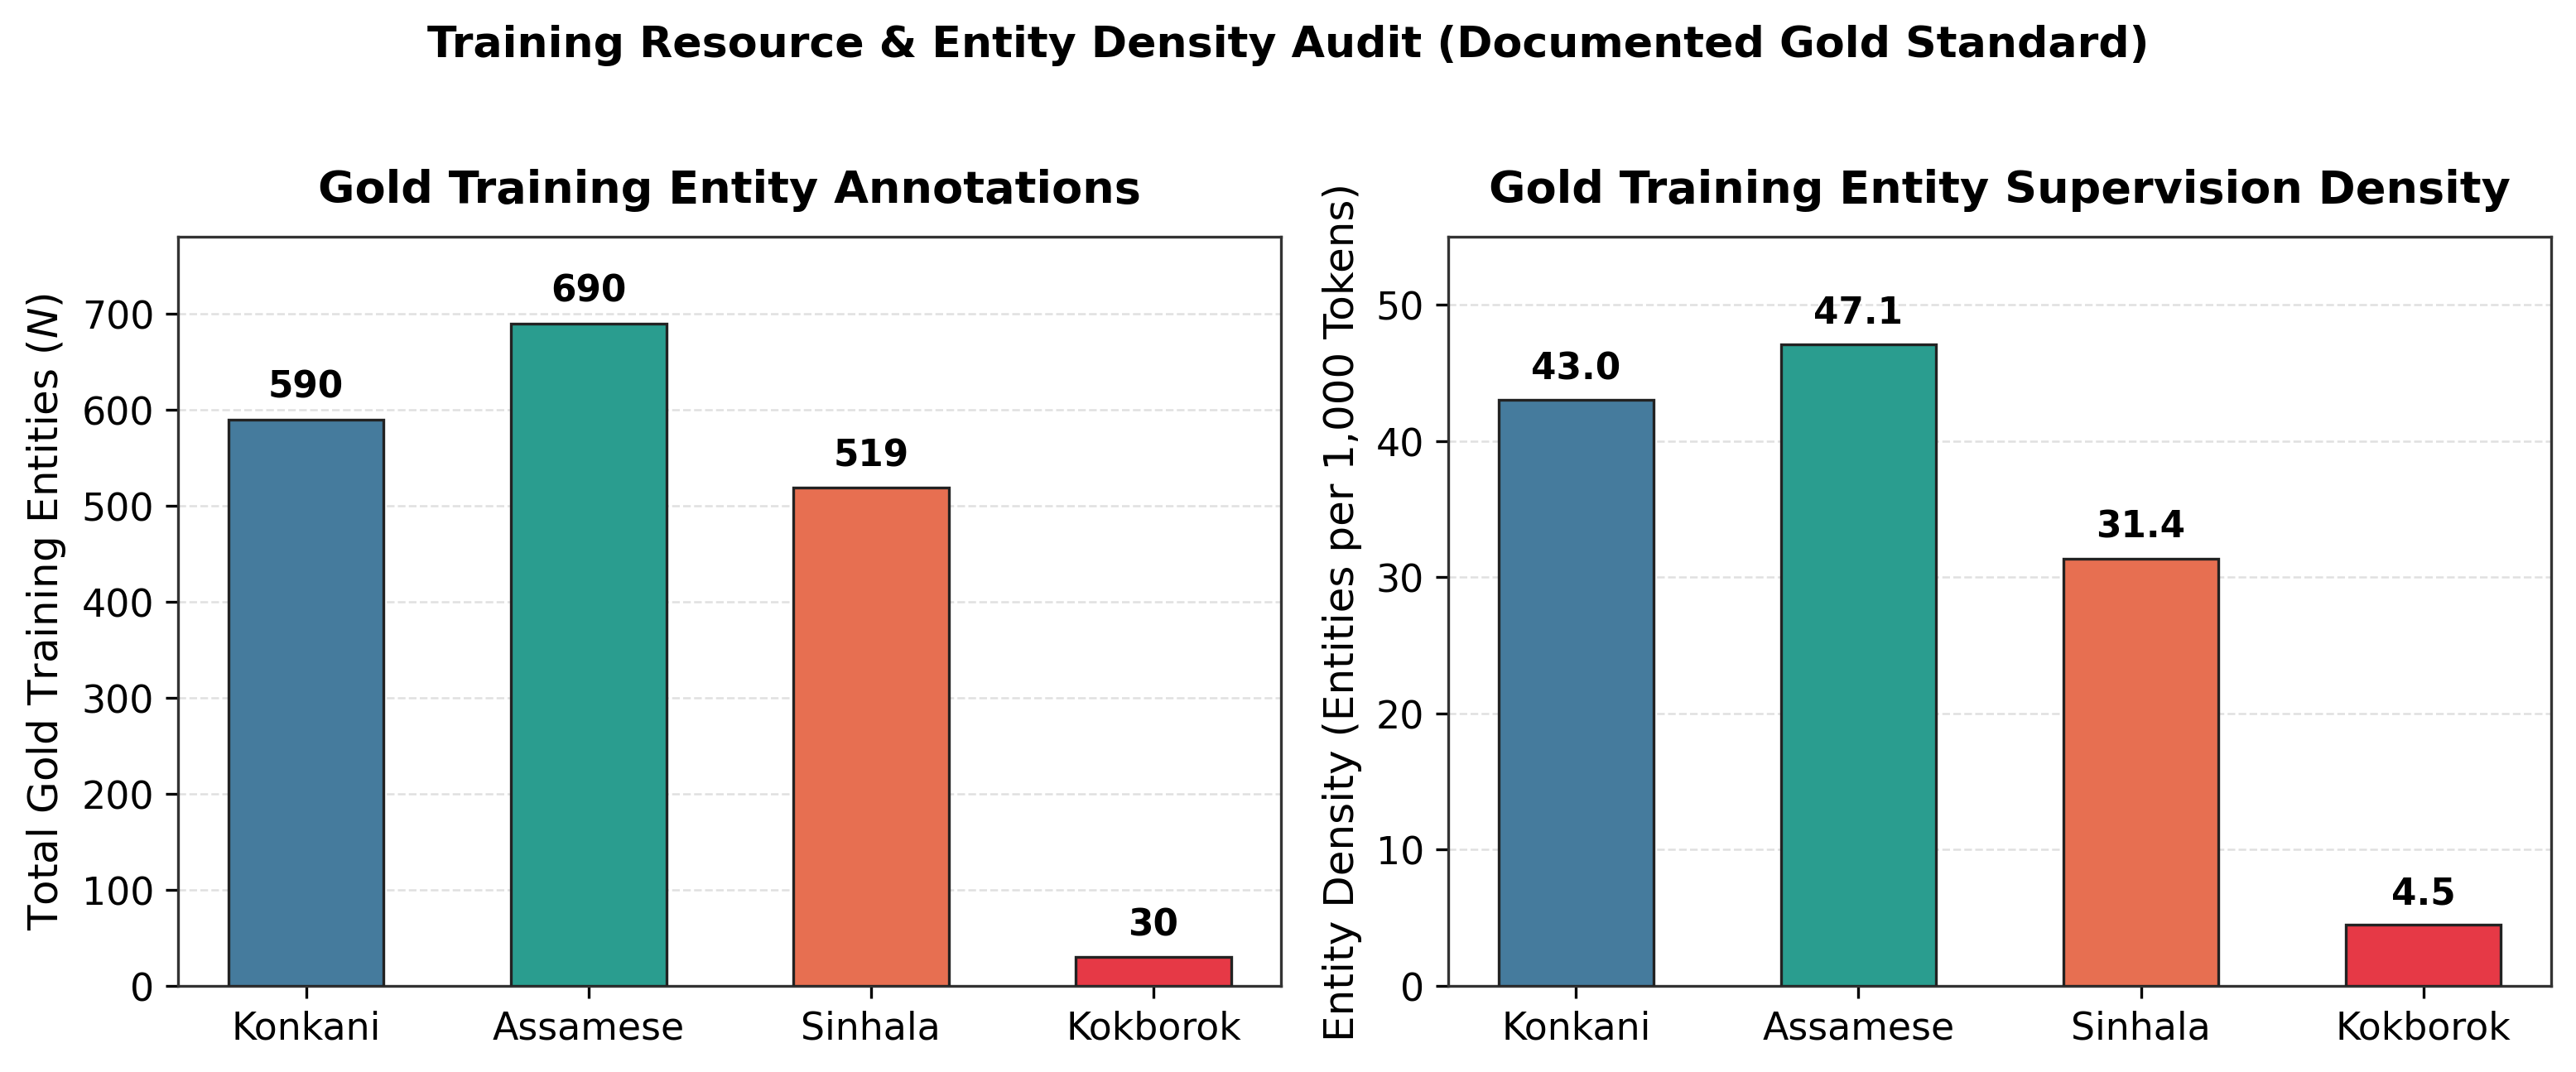
\includegraphics[width=0.92\columnwidth]{figures/fig_i_data_density.png}
\caption{Comparative audit of Gold training data resources across the four target languages: (left) total annotated entity count in the training split; (right) entity supervision density expressed as annotated entities per 1,000 training tokens.}
\label{fig:data_density}
\end{figure}

Figure~\ref{fig:data_density} shows that while the sentence count of the Gold training splits is approximately matched across languages (850 sentences for Konkani, Assamese, and Sinhala; 849 for Kokborok), the annotated entity count differs substantially. The Kokborok training split contains only 30 total annotated entity mentions across 6,711 tokens, yielding an entity density of 4.5 entities per 1,000 tokens. In contrast, the training sets for Konkani (590 entities, 13,710 tokens), Assamese (690 entities, 14,649 tokens), and Sinhala (519 entities, 16,541 tokens) provide entity densities between 31.4 and 47.1 entities per 1,000 tokens.

While unannotated Kokborok sentence pairs were gathered from public corpora (20,300 pairs) during exploratory work, automated heuristic annotations were not incorporated into the gold training standard because unverified annotations introduced boundary noise. The observed Kokborok results are consistent with the documented data-sparsity characteristics, although the present experiments do not isolate data availability from other possible factors, such as script differences or language family divergence.

\subsection{Error Analysis}\label{subsec:error_analysis}

A detailed error analysis was conducted across test set predictions to identify recurring failure patterns. Table~\ref{tab:error_analysis} summarizes the verified diagnostic cases.

\begin{table}[htbp]
\centering
\caption{Documented Error Patterns across Test Evaluations}
\label{tab:error_analysis}
\footnotesize
\setlength{\tabcolsep}{4pt}
\begin{tabular}{llp{4.2cm}p{5.0cm}}
\toprule
\textbf{Error Pattern} & \textbf{Language} & \textbf{Documented Example} & \textbf{Observed Mechanism} \\
\midrule
Boundary Truncation & Kokborok & Gold: \textit{Tripura board} (\texttt{ORG})\newline Pred: \textit{Tripura} (\texttt{LOC}) & Truncates multi-word entity; predicts only geographic base as location. \\
\midrule
Inflectional Affixation & Assamese & Locative suffix \textit{-ot} attached to location name & Attached case markers may contribute to boundary-inclusion errors. \\
\midrule
Honorific Dependency    & Konkani  & Preceding honorifics (\textit{Shri}, \textit{Dr.}) omitted in colloquial sentences & Omission of title context may contribute to false negative classifications for person names. \\
\midrule
Conjunct Corruption     & Sinhala  & Damaged touching conjuncts (\textit{bandi akshara}) & Inconsistent zero-width joiners may affect character-level representations of conjunct forms. \\
\bottomrule
\end{tabular}
\end{table}

To visualize confusion patterns across entity classes, Figure~\ref{fig:confusion_matrices} displays the test-set entity confusion matrices across the four target languages.

\begin{figure}[htbp]
\centering
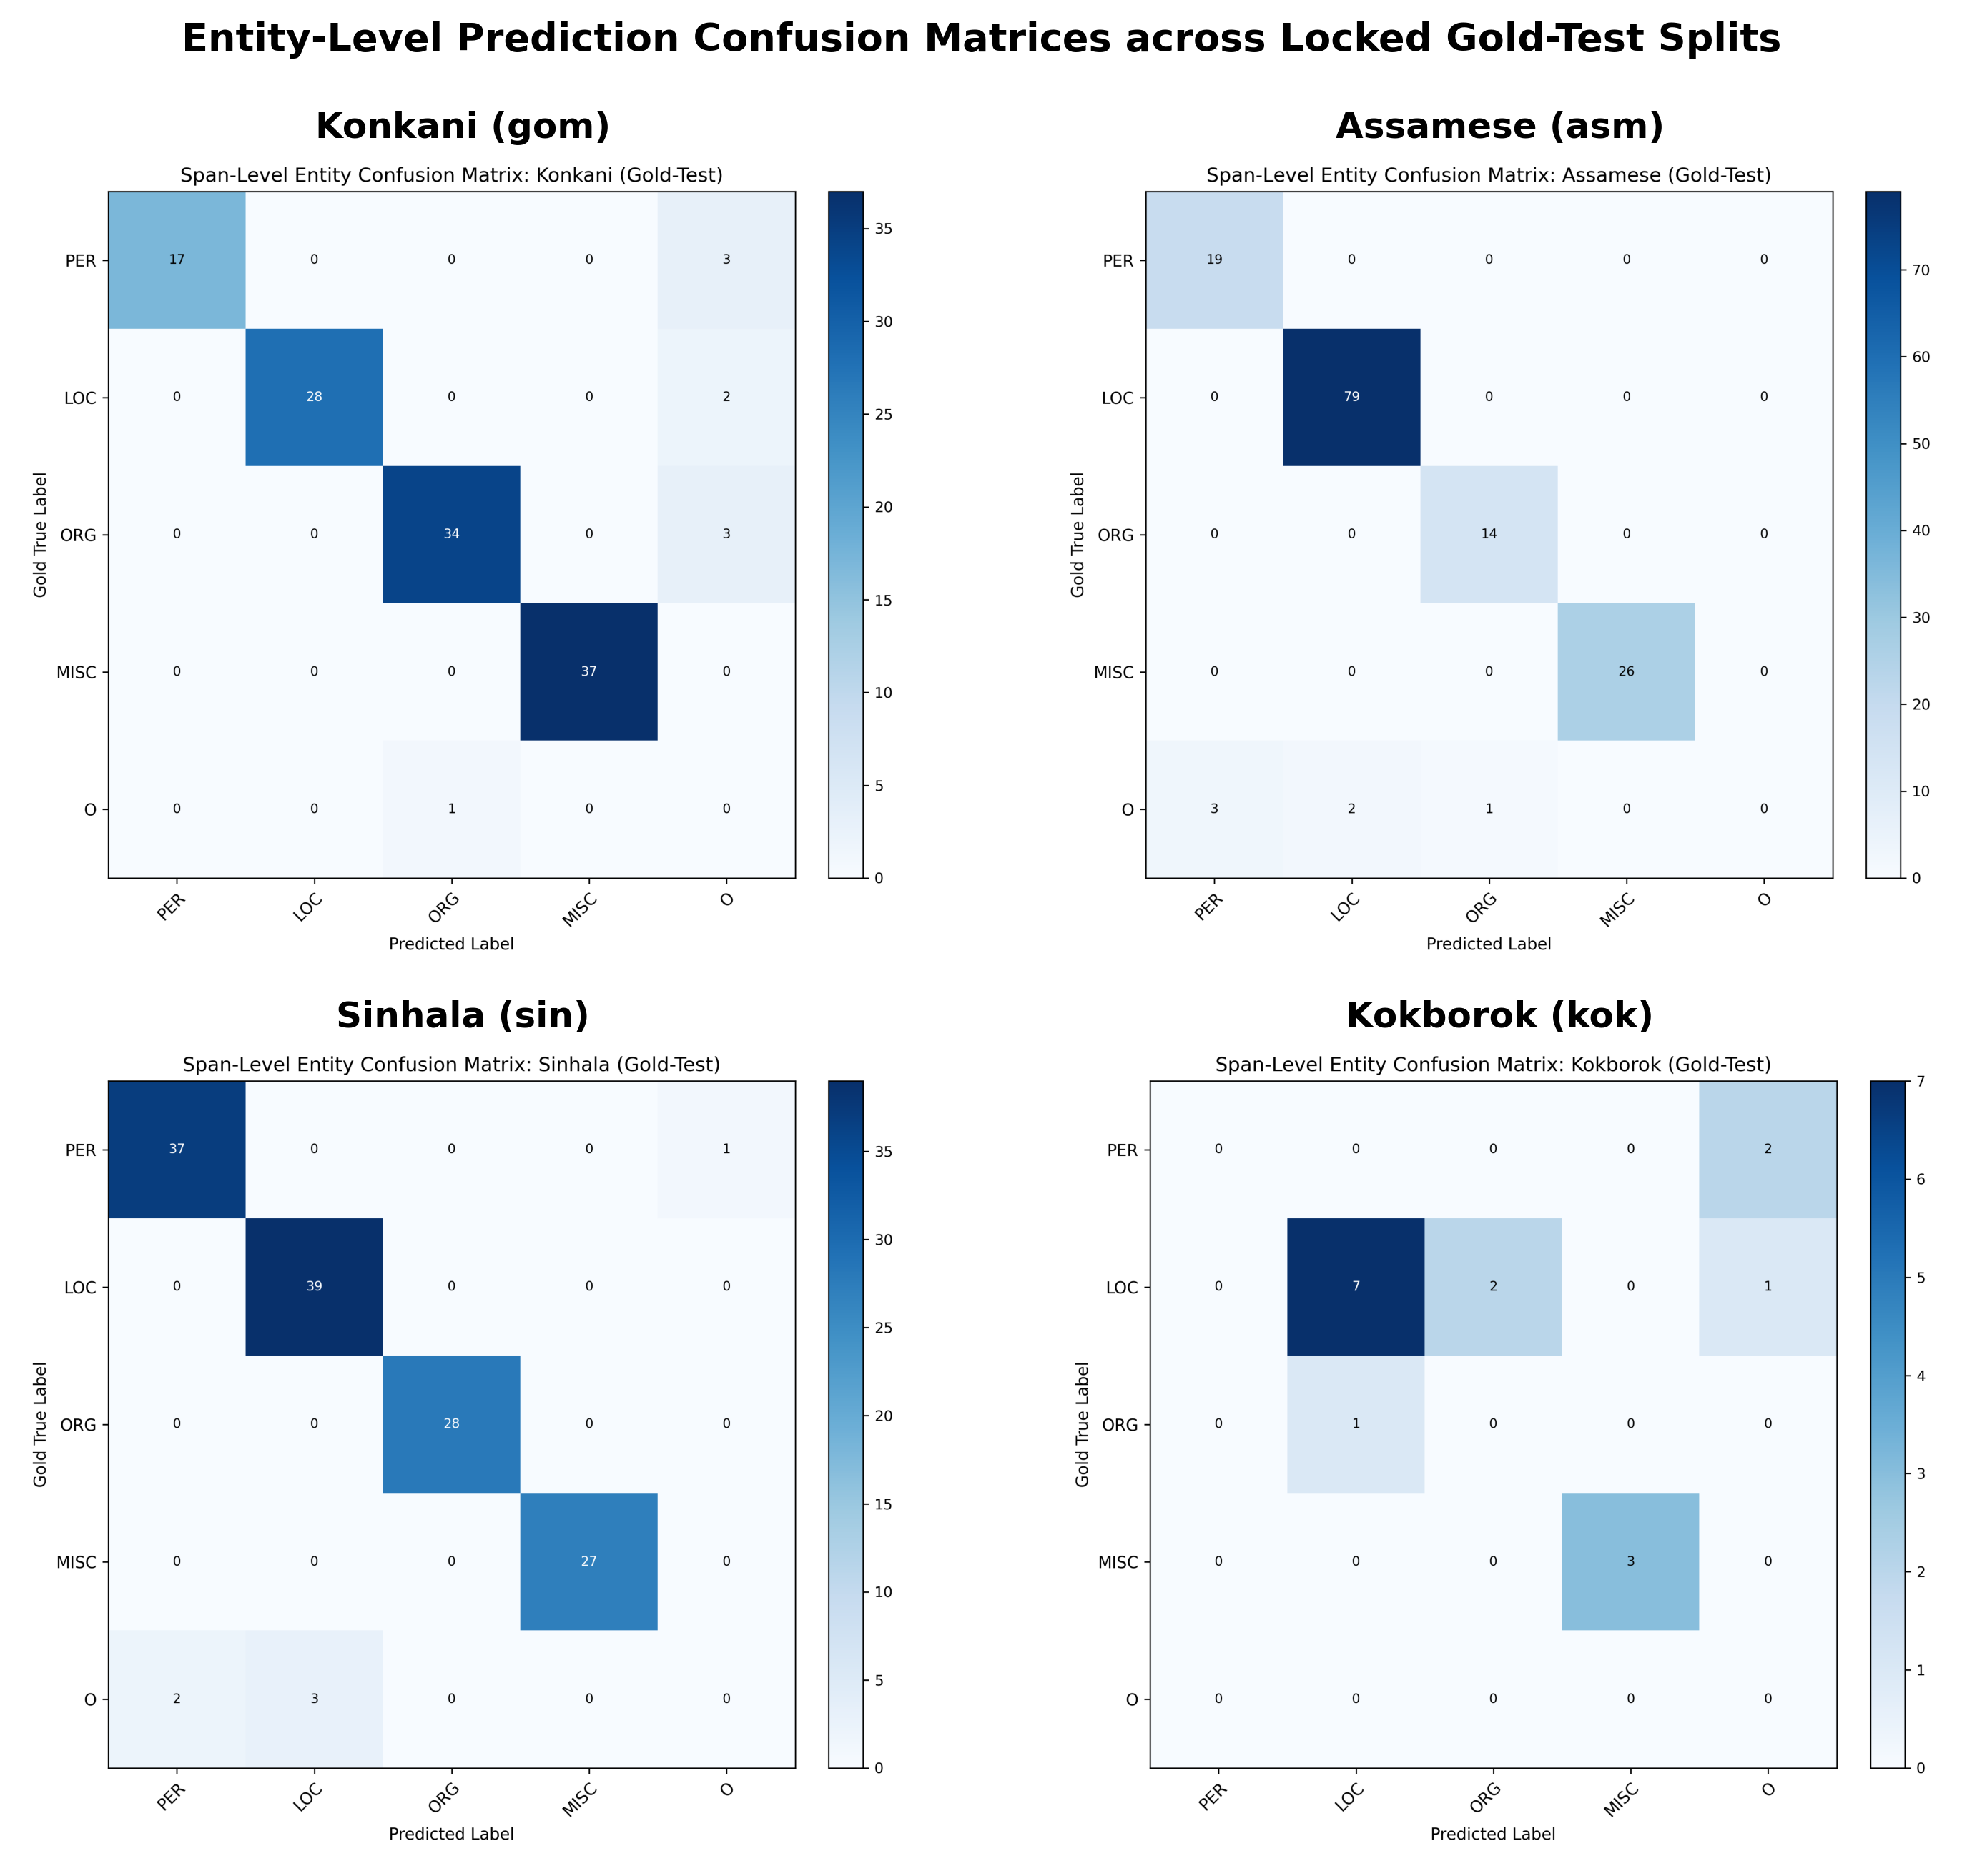
\includegraphics[width=0.82\columnwidth]{figures/fig_k_confusion_matrices.png}
\caption{Entity-level confusion matrices on the locked Gold-Test splits across Konkani, Assamese, Sinhala, and Kokborok. Diagonal entries indicate correct exact-span predictions; off-diagonal entries denote boundary mismatches or class confusions.}
\label{fig:confusion_matrices}
\end{figure}

Figure~\ref{fig:confusion_matrices} shows that classification performance is strongly diagonal for Konkani, Assamese, and Sinhala, with minor off-diagonal confusions occurring primarily between \texttt{LOC} and \texttt{ORG} categories. In Kokborok, the diagnostic failure on the entity \textit{Tripura board} illustrates boundary truncation: the model correctly recognized the geographic stem \textit{Tripura} but assigned it the \texttt{LOC} category rather than predicting the complete organizational entity \textit{Tripura board} (\texttt{ORG}). However, because only one \texttt{ORG} instance was present in the locked Kokborok test set ($N=1$), this failure represents an isolated diagnostic observation rather than a statistically representative error rate.

\subsection{Comparative Discussion with Related Literature}\label{subsec:lit_comparison}

Direct numerical comparison with published NER studies must be approached with caution. Previous research on South Asian NER has predominantly evaluated pretrained language models (such as IndicBERT, mBERT, and XLM-RoBERTa) on distinct benchmark corpora (e.g., IndicGLUE or WikiANN) that use different domain distributions, tokenization schemes, and test split partitions.

Crucially, the present work enforces a strict zero-pretrained constraint: all embeddings, CNN filters, attention matrices, and CRF transition weights are trained from scratch on at most 850 training sentences per language (850 for Konkani, Assamese, and Sinhala; 849 for Kokborok). Studies employing multilingual pretrained transformers achieve strong results by leveraging pretraining on hundreds of millions of external tokens. In contrast, our results show that a lightweight hybrid architecture combining character-level CNNs, BiLSTMs, self-attention, and a shared CRF can achieve entity F1 scores above 96\% on Konkani, Assamese, and Sinhala, and 82.35\% on Kokborok, under constrained supervision without external weights.

Furthermore, literature on attention-based sequence modeling frequently treats raw attention distributions as direct explanations of model decisions. The present attribution and erasure results support interpreting attention weights cautiously as internal information-routing signals rather than automatically treating them as faithful causal explanations.

\subsection{Integrated Discussion}\label{subsec:integrated_disc}
\enlargethispage{2\baselineskip}

The empirical findings synthesize several core insights:
\begin{enumerate}
    \item \textbf{Sequence Modeling from Scratch}: The combination of character-level grapheme representations, recurrent context modeling, multi-head attention, and global CRF decoding achieves strong entity F1 scores across diverse Brahmic and Romanized scripts without relying on external foundation models.
    \item \textbf{Divergence Between Performance and Explainability}: High sequence labeling accuracy does not guarantee that internal attention distributions provide faithful explanations. The target-token attribution audit demonstrates that the network routes information diffusely across context positions rather than concentrating on target entity tokens.
    \item \textbf{Behavioral Faithfulness Bounds}: The token-erasure benchmarks show that attribution scores reflect model sensitivity under certain conditions (as in Konkani), but can yield negative gaps when perturbation interacts with recurrent context representations (as in Assamese and Kokborok). Faithfulness evaluation must therefore be treated as an empirical behavioral test rather than proof of causal attribution.
    \item \textbf{Supervision Sensitivity}: The lower Kokborok F1 coincides with substantially lower annotated entity density, indicating that supervision availability is an important factor for further investigation. The present experiments do not isolate data availability from other possible factors.
\end{enumerate}

\section{Conclusion and Future Scope}\label{sec:conclusion}

\subsection{Conclusion}\label{subsec:conclusion}

This paper investigated explainable named entity recognition for low-resource languages under a strict from-scratch constraint. Addressing four structurally diverse languages---Konkani, Assamese, Sinhala, and Kokborok---we developed a hybrid neural architecture integrating learned word embeddings, character-level CNN grapheme representations, language conditioning vectors, bidirectional LSTMs, multi-head self-attention, and a shared linear-chain CRF decoder. By training all model parameters from scratch without external pretrained foundation models or static word vectors, the framework establishes that competitive sequence labeling can be achieved under constrained supervision.

Evaluated on cryptographically locked Gold-Test splits, the final model achieved entity F1 scores of 96.27\% in Konkani, 97.87\% in Assamese, 97.76\% in Sinhala, and 82.35\% in Kokborok, alongside token-level accuracies exceeding 99.4\% across all four languages. The comparison with the joint multilingual baseline documented consistent performance (+0.40 pp in Konkani, +0.01 pp in Assamese, and +0.72 pp in Sinhala), demonstrating the stability of the shared representation across diverse Brahmic and Romanized scripts.

Our explainability investigations provide empirical evidence regarding internal attention representations. Target-token attribution audits across correctly predicted development entities demonstrated that over 92\% of target entity tokens receive near-zero direct attribution mass ($\le 0.001$), with mean attribution ranks between 16.94 and 20.63. This indicates that high sequence labeling accuracy does not require attention weights to concentrate directly on entity query positions, consistent with the contextualized representations produced before the attention layer by the preceding two-layer BiLSTM encoder.

Subsequent token-erasure faithfulness benchmarks comparing Raw Attention and Gradient $\times$ Attention under exact CRF posterior marginals revealed divergent cross-lingual behavior: consistently positive faithfulness gaps in Konkani (+0.0127 to +0.0412) contrasted with near-zero gaps in Sinhala and negative gaps in Assamese (-0.0130 to -0.0232) and Kokborok (-0.0132 to -0.0539). These results indicate that attention distributions should not automatically be interpreted as direct causal explanations without empirical validation, as input perturbations may alter recurrently contextualized representations more broadly than specific tokens selected by post-recurrent attribution.

The comparative resource audit documented the significance of training data characteristics. Although sentence counts were matched (849 sentences in Kokborok; 850 in Konkani, Assamese, and Sinhala), Kokborok contained only 30 annotated entity mentions (4.5 entities per 1,000 tokens), compared to 519--690 entities (31.4--47.1 per 1,000 tokens) in the other three languages. This performance differential (82.35\% vs. $>96\%$) highlights the sensitivity of sequence taggers to annotated entity density, demonstrating that high token accuracy (99.55\%) can obscure the impact of acute entity sparsity. While unannotated corpora were gathered, heuristic pseudo-annotations were excluded from the gold standard to maintain annotation integrity.

From a practical and research perspective, this work demonstrates that lightweight, explainable neural sequence architectures can achieve strong labeling performance and undergo rigorous behavioral explainability auditing without relying on opaque, resource-intensive pretrained foundation models. This establishes a reproducible methodology for developing transparent sequence labeling systems in linguistically underserved communities where computational and annotated resources remain severely constrained.

\subsection{Future Scope}\label{subsec:future_scope}
\enlargethispage{3\baselineskip}

Several directions remain open for future investigation:
\begin{enumerate}
    \item \textbf{Expanded Expert Annotation}: Constructing larger, verified native-speaker annotated benchmarks for Kokborok and other underserved languages to alleviate extreme entity sparsity.
    \item \textbf{Input-Level Attribution Frameworks}: Investigating input-level attribution methods (such as Integrated Gradients) that bypass intermediate recurrent state representations to assess input-level decision faithfulness directly.
    \item \textbf{Human-Centered Interpretability}: Conducting empirical evaluations with computational linguists to determine whether post-hoc attribution signals assist human reviewers during active-learning annotation pipelines.
    \item \textbf{Controlled Pretrained Comparison}: Conducting rigorous comparative benchmarks against multilingual foundation models under strictly matched data splits and computational constraints.
\end{enumerate}

\end{document}
